\documentclass{article}
\usepackage{amsmath, amsthm, mathrsfs, graphicx}
\usepackage{amsfonts, tikz, pgf, pgfplots}

\pgfplotsset{compat=1.15}
\usetikzlibrary{arrows, positioning}
\pagestyle{empty}
\graphicspath{{C:/Users/Matej/Desktop/Personal Projects/Coursera/Complex Analysis/Notes/}}

\newtheorem{theorem}{Theorem}[section]
\newtheorem{corollary}{Corollary}[theorem]
\newtheorem{lemma}[theorem]{Lemma}
\newtheorem*{remark}{Remark}
\newtheorem{definition}{Definition}[section]
\newtheorem{conjecture}{Conjecture}[section]
%\newtheorem*{proof}{Proof}

\setcounter{tocdepth}{2}
\title{Notes on an Introduction to Complex Analysis\\
	\normalsize Based on the Introduction to Complex Analysis course on Coursera}


\begin{document}
\definecolor{ffqqqq}{rgb}{1,0,0}
\maketitle
\newpage
\tableofcontents
\newpage
\section{Complex Numbers Basics}

\subsection{Algebra and Geometry in the Complex Plane}

\subsubsection{The Complex Plane}
- Complex numbers are numbers of the form: $z = x + iy$. \\
- Set of complex numbers is denoted: $\mathbb{C}$. \\
- Real numbers are a subset of the complex numbers.

\subsubsection{Adding Complex Numbers}
Addition of complex numbers is defined as: $(x + iy) + (u+ iv) = (x + u) + i(y + v)$ \\
Thus $\Re(z + w) = \Re(z) + \Re(w)$ and $\Im(z + w) = \Im(z) + \Im(w)$

\subsubsection{The Modulus of a Complex Number}
The modulus of the complex number $z = x + iy$ is the length of the vector z:
\begin{equation*}
\left|z\right| = \sqrt{x^2 + y^2}
\end{equation*}

\subsubsection{Multiplication of Complex Numbers}
Motivation: $(x + iy)(u + iv) = xu + ixv + iyu + i^2yv$ \\
So we define:
\begin{definition}
\begin{equation*}
(x + iy)(u + iv) = (xu - yv) + i(xv + yu)
\end{equation*}
\end{definition}
The usual properties hold:
\begin{itemize}
\item $(z_1z_2)z_3 = z_1(z_2z_3)$ (associative property)
\item $z_1z_2 = z_2z_1$ (commutative property)
\item $z_1(z_2 + z_3) = z_1z_2 + z_1z_3$ (distributive property)
\end{itemize}

\subsubsection{How Do You Divide Complex Numbers?}
Suppose that $z = x +iy$ and $w = u + iv$. What is $\frac{z}{w}$(for $w \neq 0$)?
\begin{equation*}
\frac{z}{w} = \frac{x + iy}{u + iv} = \frac{(x + iy)(u - iv)}{(u + iv)(u - iv)} = \frac{xu + yv}{u^2 + v^2} + i\frac{yu - xv}{u^2 + v^2}
\end{equation*}

\subsubsection{The Complex Conjugate}
If $z = x +iy$ then $\overline{z} = x - iy$ is the complex conjugate of z. \\
Properties:
\begin{itemize}
\item $\overline{\overline{z}} = z$
\item $\overline{z + w} = \overline{z} + \overline{w}$
\item $\left|z\right| = \left|\overline{z}\right|$
\item $z\overline{z} = (x + iy)(x - iy) = x^2 + y^2 = \left|z\right|^2$
\item $\frac{1}{z} = \frac{\overline{z}}{z\overline{z}} = \frac{\overline{z}}{\left|z\right|^2}$
\end{itemize}

\subsubsection{More Properties of the Complex Conjugate}
\begin{itemize}
\item When is $z = \overline{z}$?
\item $z + \overline{z} = (x + iy) + (x - iy) = 2x$ so
\begin{equation*}
\Re(z) = \frac{z + \overline{z}}{2}, similarly \hspace{0.1cm} \Im(z) = \frac{z - \overline{z}}{2i}
\end{equation*}
\item $\left|z \cdot w\right| = \left|z\right| \cdot \left|w\right|$
\item $\overline{(\frac{z}{w})} = \frac{\overline{z}}{\overline{w}}, (w \neq 0)$
\item $\left|z\right| = 0$ if and only if $z = 0$
\end{itemize}

\subsubsection{Some Inequalities}
\begin{itemize}
\item $-\left|z\right| \leq \Re (z) \leq \left|z\right|$
\item $-\left|z\right| \leq \Im (z) \leq \left|z\right|$
\item $\left|z + w\right| \leq \left|z\right| + \left|w\right|$ (triangle inequality)
\item $\left|z - w\right| \geq \left|z\right| - \left|w\right|$ (reverse triangle inequality)
\end{itemize}

\subsubsection{The Fundamental Theorem of Algebra}
\begin{theorem}
If $a_0, a_1,..., a_n$ are complex numbers with $a_n \neq 0$, then the polynomial
\begin{equation*}
p(z) = a_nz^n + a_{n-1}z^{n-1} + ... + a_1z + a_0
\end{equation*}
has n roots $z_1, z_2,..., z_n$ in $\mathbb{C}$. It can be factored as
\begin{equation*}
p(z) = a_n(z - z_1)(z - z_2)...(z - z_n)
\end{equation*}
\end{theorem}

\subsection{Polar Representation of Complex Numbers}

\subsubsection{Polar Coordinates}
Consider a complex number $z = x + iy$. Z can also be described by the distance r from the origin and the angle $\theta$ between the positive x-axis and the line segment from 0 to z. \\
$(r, \theta)$ are the polar coordinates of z. \\
\begin{align*}
z &= x + iy \\
&= r \cos\theta + ir \sin\theta \\
&= r(\cos\theta + i \sin\theta)
\end{align*}

\subsubsection{The Argument of a Complex Number}
\begin{definition}
The principal argument of $z$, called $Arg z$, is the value of $\theta$ for which $-\pi < \theta \leq \pi$.
\end{definition}
\begin{remark}
$\theta$ is not unique! \\
$arg z = \left(Arg z + 2\pi k : k = 0, \pm 1, \pm 2,...\right), z \neq 0$
\end{remark}

\subsubsection{Exponential Notation}
Convenient notation: $e^{i\theta} = \cos\theta + i \sin\theta$ \\
So $z = r(\cos\theta + i \sin\theta)$ becomes $z = re^{i\theta}$

\subsubsection{Properties of the Exponential Notation}
\begin{itemize}
\item $\left|e^{i\theta}\right| = 1$
\item $\overline{e^{i\theta}} = e^{-i\theta}$
\item $\frac{1}{e^{i\theta}} = e^{-i\theta}$
\item $e^{i(\theta + \varphi)} = e^{i\theta} \cdot e^{i\varphi}$
\end{itemize}

\subsubsection{De Moivre's Formula}
\begin{itemize}
\item $(e^{i\theta})^n = e^{in\theta}$
\item Since $e^{i\theta} = \cos\theta + i \sin\theta$ means that: \\
$(e^{i\theta})^n = (\cos\theta + i \sin\theta)^n = \cos(n\theta) + i \sin(n\theta)$
\end{itemize}

\subsection{Roots of Complex Numbers}

\subsubsection{The nth Root}
\begin{definition}
Let $w$ be a complex number. An nth root of w is a complex number $z$ such that $z^n = w$
\end{definition}
If $w \neq 0$ there are exactly n distinct nth roots. Use the polar form for $w$ and $z$: $w = \rho e^{i\varphi} and z = re^{i\theta}$ \\
The equation $z^n = w$ then becomes
\begin{equation*}
r^ne^{in\theta} = \rho e^{i\varphi}, so \hspace{0.1cm} r^n = \rho \hspace{0.1cm} and \hspace{0.1cm} e^{in\theta} = e^{i\varphi}
\end{equation*}
Thus 
\begin{equation*}
r = \sqrt[n]{\rho} \hspace{0.1cm} and \hspace{0.1cm} n\theta = \varphi + 2k\pi, k \in \mathbb{Z}
\end{equation*}
So 
\begin{equation*}
\theta = \frac{\varphi}{n} + \frac{2k\pi}{n}, k = 0, 1,..., n-1
\end{equation*}

\subsubsection{Roots of Unity}
\begin{definition}
The nth roots of 1 are called the nth roots of unity.
\end{definition}

\subsection{Topology in the Plane}

\subsubsection{Sets in the Complex Plane}
Circles and disks: center $z_0 = x_0 + iy_0$, radius $r$.
\begin{itemize}
\item $B_{r}(z_0) = \{ z \in \mathbb{C}$ : $z$ has distance less than $r$ from $z_0 \}$ disk of radius $r$, centered at $z_0$
\item $K_{r}(z_0) = \{ z \in \mathbb{C}$ : $z$ has distance $r$ from $z_0 \}$ circle of radius $r$, centered at $z_0$
\end{itemize}
How to measure distance?
\begin{itemize}
\item
\begin{align*}
d &= \sqrt{(x - x_0)^2 + (y - y_0)^2} \\
&= \left|(x - x_0) + i(y - y_0)\right| \\
&= \left|z - z_0\right|
\end{align*}
\item So $B_r(z_0) = \{ z \in \mathbb{C} : \left|z - z_0\right| < r \}$ and $K_r(z_0) = \{ z \in \mathbb{C} : \left|z - z_0\right| = r\}$
\end{itemize}

\subsubsection{Interior Points and Boundary Points}
\begin{definition}
Let $E \subset \mathbb{C}$. A point $z_0$ is an interior point of E if there is some $r > 0$ such that $B_r(z_0) \subset E$.
\end{definition}
\begin{definition}
Let $E \subset \mathbb{C}$. A point $b$ is a boundary point of E if every disk around $b$ contains a point in E and a point not in E.
The boundary of the set $E \subset \mathbb{C}, \partial E$, is the set of all boundary points of E.
\end{definition}

\subsubsection{Open and Closed Sets}
\begin{definition}
A set $U \subset \mathbb{C}$ is open if every one of its points is an interior point.\\
A set $A \subset \mathbb{C}$ is closed if it contains all of its boundary points.
\end{definition}
Examples:
\begin{itemize}
\item $\{ z \in \mathbb{C} : \left|z - z_0\right| < r \}$ and $\{ z \in \mathbb{C} : \left|z - z_0\right| > r \}$ are open.
\item $\mathbb{C}$ and $\emptyset$ are open.
\item $\{ z \in \mathbb{C} : \left|z - z_0\right| \leq r \}$ and $\{ z \in \mathbb{C} : \left|z - z_0\right| = r \}$ are closed.
\item $\mathbb{C}$ and $\emptyset$ are closed.
\item $\{ z \in \mathbb{C} : \left|z - z_0\right| < r \} \cup \{ z \in \mathbb{C} : \left|z - z_0\right| = r$ and $\Im (z - z_0) > 0\}$ is neither open nor closed.
\end{itemize}

\subsubsection{Closure and Interior of a Set}
\begin{definition}
Let E be a set in $\mathbb{C}$. \\
The closure of E is the set E together with all of its boundary points: $\overline{E} = E \cup \partial E$. \\
The interior of E, $\mathring{E}$ is the set of all interior points of E.
\end{definition}
Examples:
\begin{itemize}
\item $\overline{B_r(z_0)} = B_r(z_0) \cup K_r(z_0) = \{ z \in \mathbb{C} : \left|z - z_0\right| \leq r \}$
\item $\overline{B_r(z_0) \setminus \{ z_0 \}} = \{ z \in \mathbb{C} : \left|z - z_0\right| \leq r \}$
\item $\overline{K_r(z_0)} = K_r(z_0)$
\item With $E = \{ z \in \mathbb{C} : \left|z - z_0\right| \leq r \}, \mathring{E} = B_r(z_0)$
\item With $E = K_r(z_0), \mathring{E} = \emptyset$
\end{itemize}

\subsubsection{Connectedness}
\begin{definition}
Two sets, X, Y in $\mathbb{C}$ are separated if there are disjoin open set U, V so that $X \subset U$ and $Y \subset V$. A set W in $\mathbb{C}$ is connected if it is impossible to find two separated non-empty sets whose union equals W.
\end{definition}
Example:
\begin{equation*}
X = [0, 1) \hspace{0.1cm} and \hspace{0.1cm} Y=(1,2]
\end{equation*}
are separated: choose $U = B_1(0)$ and $ V = B_1(2)$. Thus
\begin{equation*}
X \cup Y = [0,2] \setminus \{1\}
\end{equation*}
is not connected. It is hard to chek whether a set is connected.

\subsubsection{Connectedness for Open Sets in $\mathbb{C}$}
For open sets the is a much easier criterion to check wheter or not a set is connected:
\begin{theorem}
Let G be an open set in $\mathbb{C}$. Then G is connected if and only if any two points in G can be joined in G by successive line segments.
\end{theorem}

\subsubsection{Bounded Sets}
\begin{definition}
A set A in $\mathbb{C}$ is bounded if there exists a number $R > 0$ such that $A \subset B_R(0)$. If no such $R$ exists then $A$ is called unbounded.
\end{definition}

\section{Complex Functions, Julia Sets, Mandelbrot Set}

\subsection{Complex Functions}

\subsubsection{Functions}
\begin{itemize}
\item Recall: a function $f : A \to B$ is a rule that assigns to each element of $A$ exactly one element of B.
\item Example: $f : \mathbb{R} \to \mathbb{R}$, $f(x) = x^2 + 1$
\item Graphs help us understand the function.
\end{itemize}
\begin{figure}[h]
\centering
\begin{tikzpicture}
\begin{axis}[axis lines=left]
\addplot[color=red]{x^2+1};
\end{axis}
\end{tikzpicture}
\hskip 5 pt %ensures that the graphs are next to each other??
\begin{tikzpicture}
\begin{axis}[axis lines=left]
\addplot[color=red, samples=100]{1/(2*x^2-4};
\end{axis}
\end{tikzpicture}
\caption{$f(x) = x^2 + 1$ and $g(x) = \frac{1}{2x^2-4}$}
\end{figure}

\newpage
\subsubsection{Complex Functions}
Changing the domain and the codomain results in: $f : \mathbb{C} \to \mathbb{C}, f(z) = z^2 + 1$\\
How to graph this? 4 dimensions would be necessary, which is a bit impractical.\\
Writing $z = x + iy$ we see:
\begin{align*}
w = f(z) &= (x + iy)^2 + 1\\
&= (x^2 - y^2 + 1) + i \cdot 2xy \\
&= u(x,y) + iv(x,y)
\end{align*}
where $u,v : \mathbb{R}^2 \to \mathbb{R}$. This is one way to plot complex functions, by using two two-dimensional graphs. There is another option that is much more practical though!

\subsubsection{Graphing Complex Functions}
The idea is to consider 2 complex planes: one for the domain, and one for the range of the function. To analyze how a function behaves, we analyze how geometric configurations in the z-plane are mapped under f to the w-plane.
\begin{figure}[h]
\centering
\begin{tikzpicture}
%left graph
\draw[thick,color=blue,->] (0,0) -- (3,0);
\draw[thick,color=blue,->] (0,0) -- (0,2) node[anchor=north west] {z-plane};
\draw[thick,color=blue,->] (0,0) -- (-3,0);
\draw[thick,color=blue,->] (0,0) -- (0,-2);
%right graph
\draw[thick,color=blue,->] (7,0) -- (4,0);
\draw[thick,color=blue,->] (7,0) -- (10,0);
\draw[thick,color=blue,->] (7,0) -- (7,2) node[anchor=north east]{w-plane};
\draw[thick,color=blue,->] (7,0) -- (7,-2);
%arrow between
\draw[thick,color=black,->] (2,1) .. controls (3,2) and (4,2) .. (5,1) node[anchor=north]{$f$};
\end{tikzpicture}
\end{figure}

\subsubsection{More Complicated Functions}
How to understand more complicated functions, such as $f(z) = z^2 + c, c \in \mathbb{C}$? Same idea!
\begin{figure}[h]
\centering
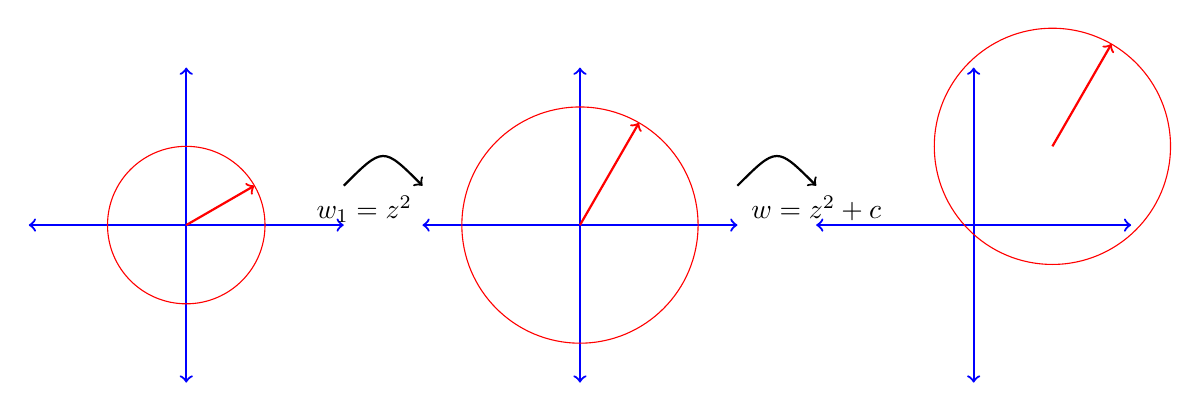
\begin{tikzpicture}
%leftmost graph
\draw[thick,color=blue,->] (0,0) -- (2,0);
\draw[thick,color=blue,->] (0,0) -- (-2,0);
\draw[thick,color=blue,->] (0,0) -- (0,2);
\draw[thick,color=blue,->] (0,0) -- (0,-2);
\draw[color=red] (0,0) circle (1cm);
\draw[thick,color=red,->] (0,0) -- (0.866,0.5);
%middle graph
\draw[thick,color=blue,->] (5,0) -- (7,0);
\draw[thick,color=blue,->] (5,0) -- (3,0);
\draw[thick,color=blue,->] (5,0) -- (5,2);
\draw[thick,color=blue,->] (5,0) -- (5,-2);
\draw[color=red] (5,0) circle (1.5cm);
\draw[thick,color=red,->] (5,0) -- (5.75,1.3);
%arrow between the leftmost and the middle one
\draw[thick,color=black,->] (2,0.5) .. controls (2.5,1) .. (3,0.5) node[anchor=north east]{$w_1=z^2$};
%rightmost graph
\draw[thick,color=blue,->] (10,0) -- (8,0);
\draw[thick,color=blue,->] (10,0) -- (12,0);
\draw[thick,color=blue,->] (10,0) -- (10,2);
\draw[thick,color=blue,->] (10,0) -- (10,-2);
\draw[color=red] (11,1) circle (1.5cm);
\draw[thick,color=red,->] (11,1) -- (11.75,2.3);
%arrow between middle and rightmost graph
\draw[thick,color=black,->] (7,0.5) .. controls (7.5,1) .. (8,0.5) node[anchor=north]{$w=z^2+c$};
\end{tikzpicture}
\end{figure}

\subsubsection{Iteration of Functions}
Let $f(z) = z +1$. \\
Then $f^2(z) = f(f(z)) = f(z+1) = (z+1) + 1= z + 2$.\\
$f^3(z) = z + 3$ \\
... $f^n(z) = z + n$ \\
$f^n$ is called the nth iterate of $f$

\subsection{Sequences and Limits of Complex Numbers}

\subsubsection{Limits}
\begin{definition}
A sequence $\{s_n\}$ of complex numbers converges to $s \in \mathbb{C}$ if for every $\epsilon > 0$ there exists an index $N \geq 1$ such that
\begin{equation*}
\left|s_n - s\right| < \epsilon \hspace{0.1cm} for \hspace{0.1cm} all \hspace{0.1cm} n \geq N
\end{equation*}
In this case we write
\begin{equation*}
\lim_{n\to\infty}\frac{1}{n}=0
\end{equation*}
\end{definition}

\subsubsection{Rules for Limits}
\begin{enumerate}
\item Convergent sequences are bounded
\item If $\{s_n\}$ converges to $s$ and $\{t_n\}$ converges to $t$, then
\begin{itemize}
\item $s_n + t_n \to s + t$
\item $s_n \cdot t_n \to s \cdot t$(in particular: $a \cdot s_n \to a \cdot s$ for any $a \in \mathbb{C}$)
\item $\frac{s_n}{t_n} \to \frac{s}{t}$, provided $t \neq 0$
\end{itemize}
\item A sequence of complex numvers, $\{s_n\}$, converges to 0 if and only if the sequence $\{\left|s_n\right|\}$ of absolute values converges to 0
\item A sequence of complex numbers, $\{s_n\}$, with $s_n = x_n + iy_n$, converges to $s = x + iy$ if and only if $x_n \to x$ and $y_n \to y$ as $n \to \infty$
\end{enumerate}

\subsubsection{Squeeze Theorem}
\begin{theorem}
Suppose that $\{r_n\},\{s_n\}$ and $\{t_n\}$ are sequences of real numbers such that $r_n \leq s_n \leq t_n$ for all $n$. If both sequences $\{r_n\}$ and $\}t_n\}$ converge to the same limit, $L$, then the sequence $\{s_n\}$ has no choice but to converge to the limit $L$ as well.
\end{theorem}
Next theorem is an equivalent of a sequence running against a wall:
\begin{theorem}
A bounded, monotone sequence of real numbers converges.
\end{theorem}

\subsubsection{Limits of Complex Functions}
\begin{definition}
$\lim_{z \to z_0} f(z) = L$ if for all $\epsilon > 0$ there exists $\delta > 0$ such that $\left|f(z) - L\right| < \epsilon$ whenever $0 < \left|z - z_0\right| < \delta$
\end{definition}

\subsubsection{Continuity}
\begin{definition}
The function $f$ is continuous at $z_0$ if $f(z) \to f(z_0)$ as $z \to z_0$
\end{definition}

\subsection{Iteration of Quadratic Polynomials, Julia Sets}

\subsubsection{Quadratic Polynomials}
Polynomials of interest are of the form $f(z) = z^2 + c$, where $c \in \mathbb{C}$ is a constant. Depending on $c$, iterates of $f$ will behave differently.\\
What about other polynomials? What about more general polynomials, $p(z) = az^2 + bz + d$, for constants $a, b, d \in \mathbb{C}$\\
As it turns out, for each triple of constants $(a, b, d)$ there is exactly one constant $c$ such that $p(z)$ and $f(z)$ behave the same under iteration\\
Why? Given $a,b$ and $d$ define $c = ad + \frac{b}{2} - (\frac{b}{2})^2$. Then letting $\phi (z) = az + b/2$ one can check that $p(z) = \phi ^{-1}(f(\phi (z)))$ for all $z$.\\
This is usually written as $p = \phi ^{-1} \circ f \circ \phi$\\
Under iteration:
\begin{align*}
p \circ p &= (\phi ^{-1} \circ f \circ \phi ) \circ (\phi ^{-1} \circ f \circ \phi ) = \phi ^{-1} \circ f \circ f \circ \phi \\
p^2 & = \phi ^{-1} \circ f^2 \circ \phi \\
p^3 &= \phi ^{-1} \circ f^3 \circ \phi \\
p^n &= \phi ^{-1} \circ f^n \circ \phi
\end{align*}

\subsubsection{The Julia Set}
The Julia set (named after the French mathematician Gaston Julia) of $f(z) = z^2 + c$ is the set of all $z \in \mathbb{C}$ for which the behaviour of the iterates is 'chaotic' in a neighbourhood. \\
The Fatou set (named after the French mathematician Pierre Fatou) is the set of all $z \in \mathbb{C}$ for thich the iterates behave 'normally' in a neighbourhood. \\
The iterates of $f$ behave normally near $z$ if nearby points remain nearby under iteration. \\
The iterates of $f$ behave chaotically at $z$ if in any small neighbourhood of $z$ the behaviour of the iterates depends sensitively on the initial point. \\
Example for the function $f(z) = z^2$ \\
The unit circle $\{z : \left|z\right| = 1\}$ is the locus of chaotic behaviour, whereas $\{z : \left|z\right| > 1\}$ (iterates attracted to $\infty$) and $\{z : \left|z\right| < 1\}$ (iterates attracted to $0$) form the locus of normal behaviour.\\
We write $J(f) = \{z : \left|z\right| = 1\}$ (Julia set) and $F(t) = \{z : \left|z\right| > 1\} \cup \{z : \left|z\right| < 1\}$ (Fatou set)

\subsubsection{The Basin of Attraction to $\infty$}
More generally, let's look at $f(z) = z^2 + c$. Let
\begin{equation*}
A(\infty) = \{z : f^n(z) \to \infty \}
\end{equation*}
'basin of attraction to $\infty$'
\begin{theorem}
The set $A(\infty)$ is open, connected and unbounded. It is contained in the Fatou set of $f$. The Julia set of $f$ coincides with the boundary of $A(\infty)$, which is a closed and bounded subset of $\mathbb{C}$.
\end{theorem}
Recap:
\begin{itemize}
\item The Julia set is a closed and bounded set.
\item The Fatou set is open and unbounded and contains $A(\infty)$.
\item Also: $J(f) \cap F(t) = \O$ and both sets are 'completely invariant' under f, meaning that $f(J) = J$ and $f(F) = F$
\end{itemize}

\subsubsection{Wrap-up}
Two examples of Julia sets:
\begin{itemize}
\item $f(z) = z^2$. $J(f) = \{z : \left|z\right| = 1\}$, the unit circle.
\item $f(z) = z^2 - 2$. $J(f) = \left[ -2, 2\right]$ the closed interval from $-2$ to $2$ on the real axis.
\end{itemize}
These two examples are only two smooth Julia sets.
\begin{figure}[h!]
\centering
\includegraphics[scale=0.5]{Julia_set_number_2.png}
\caption{$f(z) = z^2 - 2$}
\end{figure}

\subsubsection{Types of Orbits on the Julia Set of $f(z) = z^2 - 1$}
What is $J(f)$? Let's check some orbits.
\begin{itemize}
\item $z = 0: f(0) = -1, f^2(0) = f(-1) = 0, f^3(0) = f(0) = -1, f^4(0) = 0,...$ \\
The orbit is thus 0, -1, 0, -1, 0, ... \\
This is called a periodic orbit, and 0 is a periodic point of period 2. Clearly, $0 \in J(f)$.
\item $z = 1: 1, 0, -1, 0, -1, 0, -1,...$ \\
1 itself isn't a periodic point, but it runs into a periodic orbit. This is called a pre-periodic point. Again, $1 \in J(f)$
\item $z = \frac{1 + \sqrt{5}}{2}$ \\
$f(z) = (\frac{1 + \sqrt{5}}{2})^2 - 1 = \frac{1 + 2\sqrt{5} + 5}{4} - 1 = \frac{2 + 2\sqrt{5}}{4} = \frac{1 + \sqrt{5}}{2} = z$ \\
The point $\frac{1 + \sqrt{5}}{2}$ is a fixed point of $f$ and thus belongs to $J(f)$ as well.
\end{itemize}

\subsubsection{What Orbits Go Off to $\infty$?}
\begin{theorem}
Let $f(z) = z^2 + c$, and let $R = \frac{1 + \sqrt{1 + 4\left|c\right|}}{2}$. Let $z_0 \in \mathbb{C}$. If for some $n > 0$ we have that $\left|f^n(z_0)\right| > R$, then $f^n(z_0) \to \infty$ as $n \to \infty$, i.e. $z_0 \in A(\infty)$, so $z_0 \notin J(f)$
\end{theorem}

\subsubsection{The Mandelbrot Set}
\begin{definition}
The Mandelbrot set M is the set of all parameters $c \in \mathbb{C}$ for which the Julia set $J(f)$ of $f(z) = z^2 +c$ is connected.
\end{definition}
\begin{remark}
The Mandelbrot set is a subset of the parameter space (the space of all possible c-values), whereas Julia sets are sets of z-values.
\end{remark}

\subsection{The Mandelbrot Set}

\subsubsection{Finding the Mandelbrot Set}
\begin{theorem}
Let $f(z) = z^2 + c$. Then $J(f)$ is connected if and only if 0 does not belong to $A(\infty)$, that is if and only if the orbit $\{f^n(0)\}$ remains bounded under iteration.
\end{theorem}
In fact, it is possible to show the following:
\begin{theorem}
A complex number c belongs to M if and only if $\left|f^n(0)\right| \leq 2$ for all $n \geq 1$ (where $f(z) = z^2 + c$)
\end{theorem}
\begin{figure}[h]
\centering
\includegraphics[scale=0.5]{The_Mandelbrot_Set.png}
\caption{The Mandelbrot Set}
\end{figure}

\subsubsection{Properties of the Mandelbrot Set}
\begin{itemize}
\item M is a connected set.
\item M is contained in the disk of radius 2, centered at zero.
\item The boundary of M is very intricate - this is where you will find the most beautiful zooms.
\item Moreover, for c-values near the boundary of M, their Julia sets have many different patterns.
\item The boundary of the main cardioid is given by $c = \frac{1}{2}e^{i\phi} - \frac{1}{4}e^{2i\phi}, 0 \leq \phi < 2\pi$.\\
Writing $\phi = 2\pi\alpha, 0 \leq \alpha < 1$ we can distinguish whether $\alpha$ is a rational or an irrational number.
\item Rational $\alpha$: of the form $\frac{p}{q}$
\begin{itemize}
\item Example: $\alpha = \frac{1}{2}$. Then $c = \frac{1}{2}e^{\pi i} - \frac{1}{4}e^{2\pi i} = -0.75$. Here is a picture for $J(z^2 - 0.75)$:
\begin{figure}[h]
\centering
\includegraphics[scale=0.5]{Julia_set_number_3.png}
\caption{$f(z) = z^2 - 0.75$}
\end{figure}
\end{itemize}
\item Irrational $\alpha$: no values $p$ and $q$ such that $\alpha = \frac{p}{q}$.
\begin{itemize}
\item Example: $\alpha = \frac{1 + \sqrt{5}}{2}$. Then $c = -0.3905... - 0.5868...i$.
\begin{figure}[h]
\centering
\includegraphics[scale=0.5]{Julia_set_number_4.png}
\caption{Interior has a so-called 'Siegel disk'}
\end{figure}
\end{itemize}
\end{itemize}

\subsubsection{Misiurewicz Points}
A point $c \in \mathbb{C}$ is called a Misiurewicz point if the orbit of 0 under $f(z) = z^2 + c$ is pre-periodic, but not periodic.\\
Example is $c = i$.
\begin{figure}[h]
\centering
\includegraphics[scale=0.5]{Julia_set_number_5.png}
\caption{$f(z) = z^2 + i$}
\end{figure}

\subsubsection{Big Open Conjecture}
\begin{conjecture}
The Mandelbrot set is locally connected, that is, for every $c \in M$ and every open set $V$ with $c \in V$, there exists an open set $U$ such that $c \in U \subset V$ and $U \cap M$ is connected
\end{conjecture}

\section{Analytic Functions}

\subsection{The Complex Derivative}

\subsubsection{The Complex Derivative}
\begin{definition}
A complex-valued function $f$ of a complex variable is (complex) differentiable at $z_0 \in domain(f)$ if $\lim_{z \to z_0} \frac{f(z) - f(z_0)}{z - z_0}$ exists. \\
If this limit exists, it is denoted $f'(z_0)$ or $\frac{df}{dz}(z_0)$ or $\frac{d}{dz}f(z)\rvert_{z=z_0}$
\end{definition}
Example:
\begin{itemize}
\item $f(z) = c$ (a constant function, $c \in \mathbb{C}$). Let $z_0 \in \mathbb{C}$ be arbitrary. Then
\begin{equation*}
\frac{f(z) - f(z_0)}{z - z_0} = \frac{c - c}{z - z_0} = 0 \to 0 \hspace{0.1cm} as \hspace{0.1cm} z \to z_0.
\end{equation*}
Thus $f'(z) = 0$ for all $z \in \mathbb{C}$.
\end{itemize}

\subsubsection{Other Forms of the Difference Quotient}
Instead of
\begin{equation*}
\frac{f(z) - f(z_0)}{z - z_0}
\end{equation*}
we often write $z = z_0 + h$ (where $h \in \mathbb{C}$), and the difference quotient becomes
\begin{equation*}
\frac{f(z_0 + h) - f(z_0)}{h} \hspace{0.1cm} or \hspace{0.1cm} simply \hspace{0.1cm} \frac{f(z + h) - f(z)}{h}
\end{equation*}
where the limit is take as $h \to 0$. \\
Another example:
\begin{itemize}
\item $f(z) = z^2$. Then
\begin{equation*}
\frac{f(z_0 + h) - f(z_0)}{h} = \frac{(z_0 + h)^2 - z_0^2}{h} = \frac{2z_0h + h^2}{h} = 2z_0 + h \to 2z_0 \hspace{0.1cm} as \hspace{0.1cm} h \to 0.
\end{equation*}
Thus $f'(z) = 2z$ for all $z \in \mathbb{C}$.
\end{itemize}

\subsubsection{Differentiation Rules}
\begin{theorem}
Suppose $f$ and $g$ are differentiable at $z$, and $h$ is differentiable at $f(z)$. Let $c \in \mathbb{C}$.\\
Then
\begin{itemize}
\item $(cf)'(z) = cf'(z)$.
\item $(f + g)'(z) = f'(z) + g'(z)$.
\item $(f \cdot g)'(z) = f'(z)g(z) + f(z)g'(z)$.
\item $\frac{f}{g}'(z) = \frac{g(z)f'(z) - f(z)g'(z)}{(g(z))^2}, for \hspace{0.1cm} g(z) \neq 0$.
\item $(h \circ f)'(z) = h'(f(z))f'(z)$.
\end{itemize}
\end{theorem}

\subsubsection{Differentiability Implies Continuity}
\begin{theorem}
If $f$ is differentiable at $z_0$ then $f$ is continuous at $z_0$.
\end{theorem}
\begin{proof}
\begin{equation*}
\lim_{z \to z_0} (f(z) - f(z_0)) = \lim_{z \to z_0} (\frac{f(z) - f(z_0)}{z - z_0} \cdot (z - z_0)) = f'(z_0) \cdot 0 = 0
\end{equation*}
\end{proof}
\begin{remark}
Note that a function can be continuous without being differentiable.
\end{remark}

\subsubsection{Analytic Functions}
\begin{definition}
A function $f$ is analytic in an open set $U \subset \mathbb{C}$ if $f$ is (complex) differentiable at each point $z \in U$. \\
A function which is analytic in all of $\mathbb{C}$ is called an entire function.
\end{definition}
Examples:
\begin{itemize}
\item polynomials are analytic in $\mathbb{C}$ (hence entire)
\item rational functions $\frac{p(z)}{q(z)}$ are analytic wherever $q(z) \neq 0$
\item $f(z) = \overline{z}$ is not analytic
\item $f(z) = \Re z$ is not analytic
\end{itemize}

\subsection{The Cauchy-Riemann Equations}

\subsubsection{The Equations}
Recall: a complex function $f$ can be written as
\begin{equation*}
f(z) = u(x, y) + iv(x, y)
\end{equation*}
where $z = x + iy$ and $u, v$ are real-valued functions that depend on the two real variables $x$ and $y$.
\begin{theorem}
Suppose that $f(z) = u(x, y) + iv(x, y)$ is differentiable at a point $z_0$. Then the partial derivatives $u_x, u_y, v_x, v_y$ exist at $z_0$ and satisfy:
\begin{equation*}
u_x = v_y \hspace{0.1cm} and \hspace{0.1cm} u_y = -v_x
\end{equation*}
These are called the Cauchy-Riemann Equations. Also
\begin{align*}
f'(z_0) &= u_x(x_0, y_0) + iv_x(x_0, y_0) = f_x(z_0) \\
&= -i(u_y(x_0, y_0) + iv_y(x_0, y_0)) = -if_y(z_0).
\end{align*}
\end{theorem}
\begin{proof}
Suppose that $f(z) = u(x, y) + iv(x, y)$ is differentiable at a point $z_0$. Let's look at the limit definition of the derivative and take the limit as $h$ approaches $0$ along the real axis, i.e. $h = h_x + i\cdot 0$:
\begin{align*}
f'(z_0) &= \lim_{h_x \to 0} \frac{f(z_0 + h_x) - f(z_0)}{h_x}\\
&= \lim_{h_x \to 0} \frac{u(x_0 + h_x, y_0) + iv(x_0 + h_x, y_0) - u(x_0, y_0) - iv(x_0, y_0)}{h_x}\\
&= \lim_{h_x \to 0} \frac{u(x_0 + h_x, y_0) - u(x_0, y_0)}{h_x} + \lim_{h_x \to 0} i\frac{v(x_0 + h_x, y_0) - v(x_0, y_0)}{h_x}\\
&=u_x + iv_x
\end{align*}
Now let's take the limit as h approaches 0 along the imaginary axis, i.e. $h = 0 + i\cdot h_y$.
\begin{align*}
f'(z_0) &= \lim_{h_y \to 0} \frac{f(z_0 + ih_y) - f(z_0)}{ih_y}\\
&= \lim_{h_y \to 0} \frac{u(x_0, y_0 + h_y) + iv(x_0, y_0 + h_y) - u(x_0, y_0) - iv(x_0, y_0)}{ih_y}\\
&= \lim_{h_y \to 0} \frac{u(x_0, y_0 + h_y) - u(x_0, y_0)}{ih_y} + \lim_{h_y \to 0} \frac{iv(x_0, y_0 + h_y) - iv(x_0, y_0)}{ih_y}\\
&= \frac{1}{i}u_y + v_y = -iu_y + v_y
\end{align*}
For the derivative to exist, both of these limits must exist and both must be the same. Thus we can equate the two:
\begin{equation*}
-iu_y + v_y = u_x + iv_x
\end{equation*}
Equating the real and imaginary parts we get:
\begin{align*}
u_x &= v_y\\
u_y &= -v_x
\end{align*}
\end{proof}

\subsubsection{Sufficient Conditions for Differentiability}
\begin{theorem}
Let $f = u + iv$ be defined on a domain $D \subset \mathbb{C}$. Then $f$ is analytic in $D$ if and only if $u(x,y)$ and $v(x,y)$ have continuous first partial derivatives on $D$ that satisgy the Cauchy-Riemann equations.
\end{theorem}

\subsection{The Complex Exponential Function}

\subsubsection{Definition of the Complex Exponential Function}
\begin{definition}
The complex exponential function, $e^z$, sometimes also denoted $exp(z)$, is defined by 
\begin{equation*}
e^z = e^x \cdot e^{iy}, \hspace{0.1cm} where \hspace{0.1cm} z = x + iy
\end{equation*}
\end{definition}

\subsubsection{Properties of the Complex Exponential Function}
\begin{itemize}
\item $\left|e^z\right| = \left|e^x\right|\left|e^{iy}\right| = e^x$
\item $arg e^z = arg(e^xe^{iy}) = y$
\item $e^{z+2\pi i} = e^xe^{i(y+2\pi)} = e^xe^{iy} = e^z$
\item $e^{z+w} = e^ze^w$
\item $\frac{1}{e^z} = e^{-z}$
\item $e^z$ is an entire function
\item $\frac{d}{dz}e^z=e^z$
\item $\frac{d}{dz}e^{az} = a \cdot e^{az} (a \in \mathbb{C})$ by the chain rule
\item $e^{\overline{z}} = e^{x-iy} = e^xe^{-iy} = e^x\overline{e^{iy}} = \overline{e^xe^{iy}} = \overline{e^z}$
\item $e^z = 1 \iff z = 2\pi ik, k \in \mathbb{Z}$
\item $e^z = e^w \iff e^{z - w} = 1 \iff z - w = 2\pi ik \iff z = w + w\pi ik$
\end{itemize}

\subsubsection{Understanding the Mapping $w = e^z$}
The function $w = e^z$ is a mapping from $\mathbb{C} \to \mathbb{C}$. \\
Let's map horizontal lines of the form $L = \{x + iy_0 \| x\in \mathbb{R} \}$ for fixed $y_0 \in \mathbb{R}$.
\begin{figure}[h]
\centering
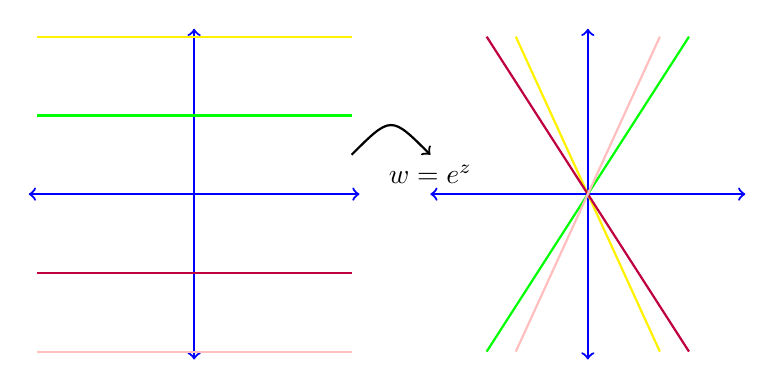
\begin{tikzpicture}
%left coordinate axes
\draw[thick,color=blue,->] (0,0) -- (2.1,0);
\draw[thick,color=blue,->] (0,0) -- (0,2.1);
\draw[thick,color=blue,->] (0,0) -- (0,-2.1);
\draw[thick,color=blue,->] (0,0) -- (-2.1,0);
%horizontal lines
\draw[thick,color=yellow] (-2,2) -- (2,2);
\draw[thick,color=green] (-2,1) -- (2,1);
\draw[thick,color=purple] (-2,-1) -- (2,-1);
\draw[thick,color=pink] (-2,-2) -- (2,-2);
%right coordinate axes
\draw[thick,color=blue,->] (5,0) -- (3,0);
\draw[thick,color=blue,->] (5,0) -- (7,0);
\draw[thick,color=blue,->] (5,0) -- (5,2.1);
\draw[thick,color=blue,->] (5,0) -- (5,-2.1);
%transformed horizontal lines
\draw[thick,color=yellow] (4.085,2) -- (5.915,-2);
\draw[thick,color=green] (6.285,2) -- (3.715,-2);
\draw[thick,color=purple] (3.715,2) -- (6.285,-2);
\draw[thick,color=pink] (5.915,2) -- (4.085,-2);
%arrow between
\draw[thick,color=black,->] (2,0.5) .. controls (2.5,1) .. (3,0.5) node[anchor=north]{$w = e^z$};
\end{tikzpicture}
\end{figure}
Let's now map vertical lines of the form $L = \{x_0 + iy \| y \in \mathbb{R} \}$ for fixed $x_0 \in \mathbb{R}$
\begin{figure}[h]
\centering
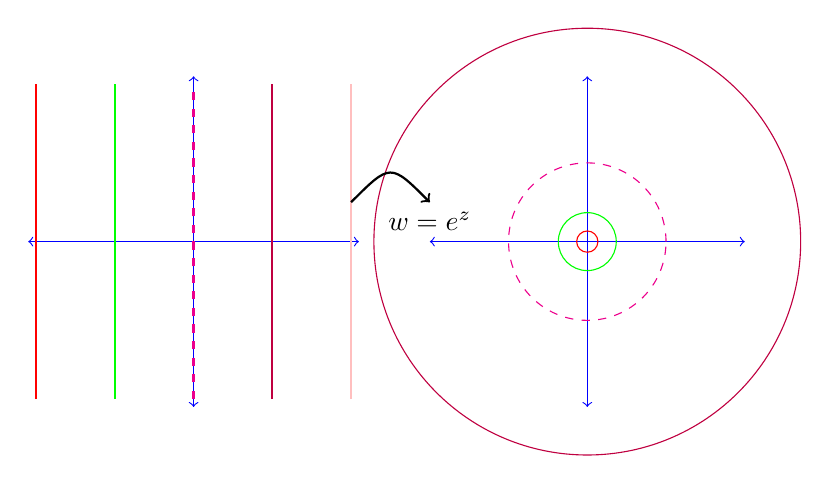
\begin{tikzpicture}
%left coordinate axes
\draw[thin,color=blue,->] (0,0) -- (2.1,0);
\draw[thin,color=blue,->] (0,0) -- (0,2.1);
\draw[thin,color=blue,->] (0,0) -- (0,-2.1);
\draw[thin,color=blue,->] (0,0) -- (-2.1,0);
%vertical lines
\draw[thick,color=red] (-2,-2) -- (-2,2);
\draw[thick,color=green] (-1,-2) -- (-1,2);
\draw[thick,color=purple] (1,-2) -- (1,2);
\draw[thick,color=pink] (2,-2) -- (2,2);
\draw[dashed,thick,color=magenta] (0,-2) -- (0,2);
%right coordinate axes
\draw[thin,color=blue,->] (5,0) -- (3,0);
\draw[thin,color=blue,->] (5,0) -- (7,0);
\draw[thin,color=blue,->] (5,0) -- (5,2.1);
\draw[thin,color=blue,->] (5,0) -- (5,-2.1);
%lines transformed to circles
\draw[color=red] (5,0) circle (0.135cm);
\draw[color=green] (5,0) circle (0.368cm);
\draw[color=purple] (5,0) circle (2.71cm);
\draw[dashed,color=magenta] (5,0) circle (1cm);
%arrow between
\draw[thick,color=black,->] (2,0.5) .. controls (2.5,1) .. (3,0.5) node[anchor=north]{$w = e^z$};
\end{tikzpicture}
\end{figure}

\subsection{Complex Trigonometric Functions}

\subsubsection{Definition}
Having extended the exponential function to the complex plane, can the same be done for the trigonometric functions?
\begin{definition}
The complex cosine and sine dunctions are defined vie
\begin{equation*}
\cos z = \frac{e^{iz} + e^{-iz}}{2} \hspace{0.1cm} and \hspace{0.1cm} \sin z = \frac{e^{iz} - e^{-iz}}{2i}
\end{equation*}
\end{definition}

\subsubsection{Properties}
\begin{itemize}
\item $\sin z$ and $\cos z$ are analytic functions (in fact, entire).
\item For real-valued z (i.e. $z = x + i \cdot 0$) the complex sine and cosine agree with the real-valued sine and cosine functions.
\item $\cos (-z) = \frac{e^{-iz} + e^{iz}}{2} = \cos z$.
\item $\sin (-z) = \frac{e^{-iz} - e^{iz}}{2i} = - \sin z$
\item $\cos (z + w) = \cos z \cos w - \sin z \sin w$, \\
$\sin (z + w) = \sin z \cos w + \cos z \sin w$.
\item $\cos (z + 2\pi) = \cos z$ \\
$\sin (z + 2\pi) = \sin z$
\item $\sin^2z + \cos^2z = 1$
\item $\sin (z + \frac{\pi}{2} = \cos z$
\end{itemize}

\subsubsection{The Zeros of Sine and Cosine}
$\sin z = 0 \iff z = k\pi, k \in \mathbb{Z}$ \\
$\cos z = 0 \iff z = \frac{\pi}{2} + k\pi, k \in \mathbb{Z}$

\subsubsection{Relation to Hyperbolic Functions}
$\sin z = \sin x \cosh y + i \cos x \sinh y$ \\
$\cos z = \cos x \cosh y - i \sin x \sinh y$

\subsection{First Properties of Analytic Functions}

\subsubsection{Analytic Functions with Zero Derivative}
\begin{theorem}
If $f$ is analytic on a domain $D$, and if $f'(z) = 0$ for all $z\in D$, then $f$ is constant in $D$.
\end{theorem}
\begin{remark}
Recall the 1-dimension analog: \\
If $f : (a, b) \to \mathbb{R}$ is differentiable and satisfies $f'(x) = 0$ for all $x \in (a, b)$, then $f$ is constant on $(a, b)$.
\end{remark}
\begin{proof}
First step of the proof:
\begin{itemize}
\item
Let $B_r(a)$ be a disk contained in $D$, and let $c \in B_r(a)$. Pick the point $b \in B_r(a)$ as in the figure.
\begin{figure}[h!]
\centering
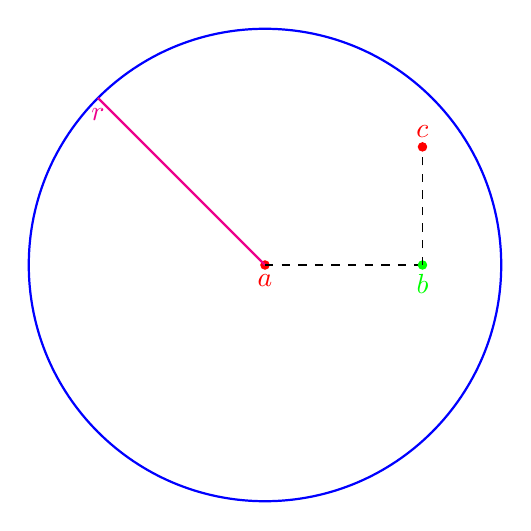
\begin{tikzpicture}
\draw[thick,color=blue] (0,0) circle (3cm);
\draw[color=red,fill] (0,0) circle (1.5pt) node[anchor=north]{$a$};
\draw[thick,color=magenta] (0,0) -- (-2.1213,2.1213) node[anchor=north] {$r$};
\draw[dashed,color=black] (0,0) -- (2,0);
\draw[color=green,fill] (2,0) circle (1.5pt) node[anchor=north]{$b$};
\draw[dashed,color=black] (2,0) -- (2,1.5);
\draw[color=red,fill] (2,1.5) circle (1.5pt) node[anchor=south]{$c$};
\end{tikzpicture}
\caption {First part of the proof}
\end{figure}
Since $f'(z) = 0$ in $D$ we have $u_x = u_y = v_x = v_y = 0$ in $D$. In particular, look at $u$ on the horizontal line segment from $a$ to $b$. It depends only on one parameter (namely $x$) there, and $u_x = 0$. By the 1-dimensional fact, we find that $u$ is constant on the line segment, in particular, $u(a) = u(b)$. Similarly, $u(b) = u(c)$, thus $u(a) = u(c)$. Since $c$ was an arbitrary point in $b_r(a)$, $u$ is thus constant in $B_r(a)$. Similarly, $v$, is constant in $B_r(a)$, thus $f$ is constant in $B_r(a)$.
\end{itemize}
Here is the second step of the proof:
\begin{itemize}
\item Let $a$ and $b$ be two arbitrary points in $D$. Since $D$ is connected, there exists a nice curve in $D$, joining $a$ and $b$.
\begin{figure}[h!]
\centering
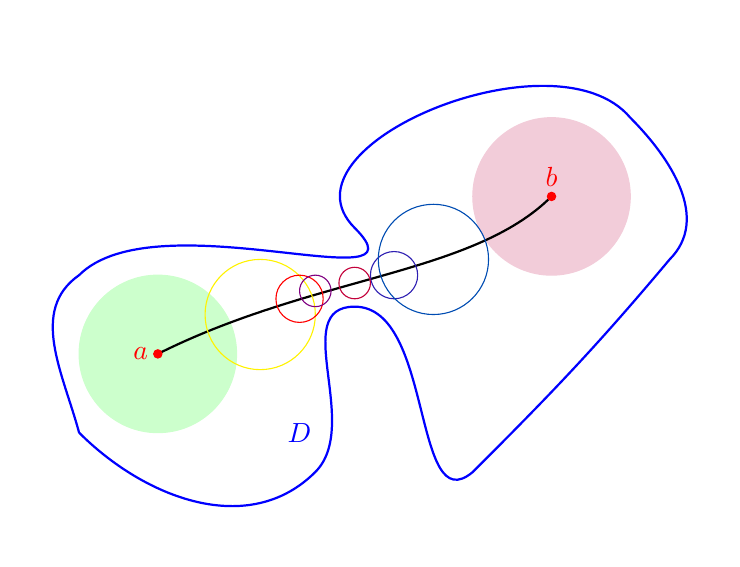
\begin{tikzpicture}
%End circles and the line in between
\draw[fill,color=green!20] (0,0) circle (1cm);
\draw[fill,color=purple!20] (5,2) circle (1cm);
\draw[thick,color=black] (0,0) .. controls (2,1) and (4,1) .. (5,2);
\draw[fill,color=red] (0,0) circle (1.5pt) node[anchor=east]{$a$};
\draw[fill,color=red] (5,2) circle (1.5pt) node[anchor=south]{$b$};
%circles on the line
\draw[color=yellow] (1.3,0.5) circle (0.7cm);
\draw[color=red] (1.8,0.7) circle (0.3cm);
\draw[color=red!50!blue] (2,0.8) circle (0.2cm);
\draw[color=red!60!green!30!blue] (3,1) circle (0.3cm);
\draw[color=green!30!blue] (3.5,1.2) circle(0.7cm);
\draw[color={rgb:red,213;green,1;blue,65}] (2.5, 0.9) circle(0.2cm);
%blue line outside
\draw[thick,color=blue] (-1,-1) to [out=315, in=225] (2,-1.5)
							to [out=45, in=180] (2.5,0.6)
							to [out=0, in=220] (4,-1.5)
							to [out=45, in=230] (6.5,1.2)
							to [out=45, in=315] (6,3)
							to [out=130, in=135] (2.5, 1.6)
							to [out=315, in = 45] (-1,1)
							to [out=215, in=105] (-1,-1);
\node[color=blue] at (1.8,-1) {$D$};
\end{tikzpicture}
\caption{Second Part of the proof}
\end{figure}
By the previous step, $f$ is constant in the disk around the point $a$ (see picture). Furthermore, $f$ is also constant in the neighbouring disk. Since these two disks overlap, the two constants must agree. Continue on in this matter until you reach $b$. Therefore, $f(a) = f(b)$. Thus $f$ is constant in $D$.
\end{itemize}
\end{proof}

\subsubsection{Consequences}
The previous theorem, together with the Cauchy-Riemann equations, has strong consequences.
\begin{itemize}
\item Suppose that $f = u + iv$ is analytic in a domain $D$. Suppose furthermore, that $u$ is constant in $D$. Then $f$ must be constant in $D$.
\begin{proof}
$u$ constant in $D$ implies that $u_x = u_y = 0$ in $D$. Since $f$ is analytic, the Cauchy-Riemann equations now imply that $v_x = v_y = 0$ as well. Thus $f' = u_x + iv_x = 0$ in $D$. By previous theorem, $f$ is constant in $D$.
\end{proof}
\item Similarly, if $f = u + iv$ is analytic in a domain $D$ with $v$ being constant, then $f$ must be constant in $D$.
\item Suppose next that $f = u + iv$ is analytic in a domain $D$ with $\left|f\right|$ being constant in $D$. This too implies that $f$ itself must be constant
\begin{proof}
Let $f = u + iv$ be analytic in a domain $D$, and suppose that $\left|f\right|$ is constant in $D$. Then $\left|f\right|^2$ is also constant, i.e. there exists $c \in \mathbb{C}$ such that
\begin{equation*}
\left|f(z)\right|^2 = u^2(z) + v^2(z) = c \hspace{0.1cm} for \hspace{0.1cm} all \hspace{0.1cm} z \in D.
\end{equation*}
\begin{itemize}
\item If $c = 0$ then $u$ and $v$ must be equal to zero everywhere, and so $f$ is equal to zero in $D$.
\item If $c \neq 0$ then in fact $c > 0$. Taking the partial derivative with respect to $x$ (and similarly with respect to $y$) of the above equation yields:
\begin{equation*}
2uu_x + 2vv_x = 0 \hspace{0.1cm} and \hspace{0.1cm} 2uu_y = 2vv_y = 0
\end{equation*}
Substituting $v_x = -u_y$ in the first and $v_y = u_x$ in the second equation gives
\begin{equation*}
uu_x - vu_y = 0 \hspace{0.1cm} and \hspace{0.1cm} uu_y + vu_x = 0.
\end{equation*}
Multiplying the first equation by $u$ and the second by $v$ we find
\begin{equation*}
u^2u_x - uvu_y = 0 \hspace{0.1cm} and \hspace{0.1cm} uvu_y + v^2u_x = 0.
\end{equation*}
Add the two equations.
\begin{equation*}
u^2u_x + v^2u_x = 0
\end{equation*}
Since $u^2 + v^2 = c$, this last equation becomes
\begin{equation*}
cu_x = 0
\end{equation*}
But $c > 0$, so it must be the case that $u_x = 0$ in $D$. We can similarly find that $u_y = 0$ in $D$, and using the Cauchy-Riemann equations we also obtain that $v_x = v_y = 0$ in $D$. Hence $f'(z) = 0$ in $D$, and the theorem yields that $f$ is constant in $D$.
\begin{remark}
The assumption of D being connected is important!
\end{remark}
\end{itemize}
\end{proof}
\end{itemize}

\subsection{Inverse Functions of Analytic Functions}
\subsubsection{The Logarithm Function}
\begin{definition}
For $z \neq 0$ we define 
\begin{equation*}
Log z = ln \left|z\right| + i Arg z, \hspace{0.1cm} the principal branch of logarithm,
\end{equation*}
and
\begin{align*}
log z &= ln \left|z\right| + i arg z, \hspace{0.1cm} a \hspace{0.1cm} multi-valued \hspace{0.1cm} function \\
&= Log z + 2k\pi i, k \in \mathbb{Z}.
\end{align*}
\end{definition}

\subsubsection{Continuity of the Logarithm Function}
Notice:
\begin{itemize}
\item $z \mapsto \left|z\right|$ is continuous in $\mathbb{C}$.
\item $z \mapsto ln\left|z\right|$ is continuous in $\mathbb{C} \backslash \{0\}$.
\item $z \mapsto Arg z$ is continous in $\mathbb{C} \backslash (-\infty, 0]$
\item Thus, $Log z$ is continuous in $\mathbb{C} \backslash (-\infty, 0]$.
\item However, as $z \to -x \in (-\infty, 0)$ from above, $Log z \to ln x + i\pi$, and as $z \to -x$ from below, $Log z \to ln x - i\pi$, so $Log z$ is not continuous on $(-\infty, 0)$ (and not defined at 0).
\end{itemize}
Fact: The principal branch of logarithm, $Log z$, is analytic in $\mathbb{C} \backslash (-\infty, 0]$.

\subsubsection{Theorem about Finding Derivatives of Functions}
\begin{theorem}
Suppose that $f : U \to \mathbb{C}$ is an analytic function and there exists a continuous function $g : D \to U$ from some domain $D \in \mathbb{C}$ into $U$ such that $f(g(z)) = z$ for all $z \in D$. Then $g$ is analytic in $D$, and
\begin{equation*}
g'(z) = \frac{1}{f'(g(z))} \hspace{0.1cm} for \hspace{0.1cm} z \in D.
\end{equation*}
\end{theorem}
\subsubsection{Application 1}
Let $f : \mathbb{C} \to \mathbb{C}, f(z) = z^2.$ Then $f'(z) = 2z$. \\
Let $g : \mathbb{C} \backslash (-\infty, 0] \to \mathbb{C}, g(z) = \sqrt{z}$ be the principal branch of the square root. \\
Then
\begin{itemize}
\item $f(g(z)) = z$ for all $z \in D = \mathbb{C} \backslash (-\infty, 0]$
\item $g$ is continuous in $D$, thus $g$ is analytic in D, and
\begin{align*}
g'(z) &= \frac{1}{f'(g(z))} \\
&= \frac{1}{2\sqrt{z}}
\end{align*}
\end{itemize}

\subsubsection{Some Terminology}
Let $f : U \to V$ be a function.
\begin{itemize}
\item $f$ is injective (also called 1-1) provided that $f(a) \neq f(b)$ whenever $a,b \in U$ with $a \neq b$.
\item $f$ is surjective (also called onto) provided that for every $y \in V$ there exists and $x \in U$ such that $f(x) = y$.
\item $f$ is a bijection (also called 1-1 and onto) if $f$ is both injective and surjective.
\end{itemize}

\subsection{Conformal Mappings}
\subsubsection{What is a Conformal Mapping}
Inuitively, a conformal mapping is a mapping that preserves the angles between curves.
\begin{figure}[h]
\centering
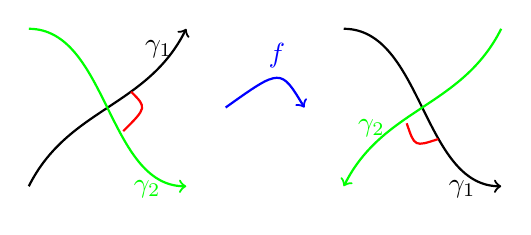
\begin{tikzpicture}
%left lines
\draw[thick,color=black,->] (-1,-1) .. controls (-0.5,0) and (0.5,0) .. (1,1) node[pos=0.8,above] {$\gamma_1$};
\draw[thick,color=green,->] (-1,1) .. controls (0,1) and (0,-1) .. (1,-1) node[pos=0.8,below] {$\gamma_2$};
\draw[thick,color=red] (0.2,-0.3) .. controls (0.5,0) .. (0.3,0.2);
%arrow
\draw[thick,color=blue,->] (1.5,0) .. controls (2.2,0.5) .. (2.5,0) node[pos=0.5,above] {$f$};
%right lines
\draw[thick,color=black,->] (3,1) .. controls (4,1) and (4,-1) .. (5,-1) node[pos=0.8,below] {$\gamma_1$};
\draw[thick,color=green,->] (5,1) .. controls (4.5,0) and (3.5,0) .. (3,-1) node[pos=0.8,above] {$\gamma_2$};
\draw[thick,color=red] (3.8, -0.2) .. controls (3.9,-0.5) .. (4.2, -0.4);
\end{tikzpicture}
\end{figure}

\subsubsection{Paths}
\begin{definition}
A path in the complex plane from a point $A$ to a point $B$ is a continuous function $\gamma : [a, b] \to \mathbb{C}$ such that $\gamma (a) = A$ and $\gamma (b) = B$.
\end{definition}

\subsubsection{Curves}
\begin{definition}
A path $\gamma : [a, b] \to \mathbb{C}$ is smooth if the functions $x(t)$ and $y(t)$ in the representation $\gamma (t) = x(t) + iy(t)$ are smooth, that is, have as many derivatives as desired.
\end{definition}

\subsubsection{The Angle Between Curves}
\begin{definition}
Let $\gamma_1$ and $\gamma_2$ be two smooth curves, intersecting at a point $z_0$. The angle between the two curves at $z_0$ is defined as the angle between the two tangent vectors at $z_0$.
\end{definition}

\subsubsection{Conformality}
\begin{definition}
A function is conformal if it preserves angles between curves. More precisely, a smooth complex-valued function $g$ is conformal at $z_0$ if whenever $\gamma_1$ and $\gamma_2$ are two curves that intersect at $z_0$ with non-zero tangents, then $g \circ \gamma_1$ and $g \circ \gamma_2$ have non-zero tangents at $g(z_0)$ that intersect at the same angle.\\
A conformal mapping of a domain $D$ onto $V$ is a continuously differentiable mapping that is conformal at each point in $D$ and maps $D$ one-to-one onto $V$.
\end{definition}

\subsubsection{Analytic Functions}
\begin{theorem}
If $f : U \to \mathbb{C}$ is analytic and if $z_0 \in U$ such that $f'(z_0) \neq 0$, then $f$ is conformal at $z_0$.
\end{theorem}

\subsection{Mobius Transformations}
\subsubsection{Mobius Transformations}
\begin{definition}
A Mobius transformation (also called fractional linear transformation) is a function of the form
\begin{equation*}
f(z) = \frac{az + b}{cz + d},
\end{equation*}
where $a, b, c, d \in \mathbb{C}$ such that $ad - bc \neq 0$.
\end{definition}
Notes:
\begin{itemize}
\item As $z \to \infty$, $f(z) \to \frac{a}{c}$ if $c \neq 0$ and $f(z) \to \infty$ if $c = 0$. \\
That's why $z = \infty$ is allowed and $f(\infty) = \frac{a}{c}$ is defined if $c \neq 0$ and $f(\infty) = \infty$ if $c = 0$.
\item Similarly, $f(-\frac{d}{c}) = \infty$, if $c \neq 0$.
\item We thus regard $f$ as a mapping from the extended complex plane $\hat{\mathbb{C}} = \mathbb{C} \cup \{ \infty \} $ to the extended plane $\hat{\mathbb{C}}$.
\end{itemize}

\subsubsection{Properties of $f(z) = \frac{az + b}{cz + d}, a, b, c, d \in \mathbb{C}, ad - bc \neq 0$}
\begin{itemize}
\item $f'(z) = \frac{(cz + d)a - (az + b)c}{(cz + d)^2} = \frac{ad - bc}{(cz + d)^2}$. The condition $ad - bc \neq 0$ thus simply guarantees that $f$ is non-constant.
\item If we multiply each parameter of $a, b, c, d$ by a constant $k \neq 0$, we obtain the same mapping, so a given mapping does not uniquely determine $a, b, c, d$.
\item A Mobius transformation is one-to-one and onto from $\hat{\mathbb{C}}$ to $\hat{\mathbb{C}}$.
\begin{proof}
Pick $w \in \hat{\mathbb{C}}$ and observe
\begin{align*}
f(z) = w &\iff az + b = w(cz + d) \\
&\iff z(a - wc) = wd - b \\
&\iff z = \frac{wd - b}{-wc + a}
\end{align*}
For each $w \in \hat{\mathbb{C}}$ there is one and only one $z \in \hat{\mathbb{C}}$ such that $f(z) = w$.
\end{proof}
\end{itemize}

\subsubsection{Conformality of $f(z) = \frac{az + b}{cz + d}, a, b, c, d \in \mathbb{C}, ad - bc \neq 0$}
Mobius transformations are thus conformal mappings from $\hat{\mathbb{C}}$ to $\hat{\mathbb{C}}$. In fact, Mobius transformations are the only conformal mappings from $\hat{\mathbb{C}}$ to $\hat{\mathbb{C}}$.

\subsubsection{The Inversion $f(z) = \frac{1}{z}$}
Let $K = \{z : \left|z - 3\right| = 1 \}$ be the circle of radius $1$, centered at $3$.
\begin{align*}
w \in f(K) \iff \frac{1}{w} \in K &\iff \left| \frac{1}{w} - 3 \right| = 1\\
&\iff \left|1 - 3w\right|^2 = \left|w\right|^2\\
&\iff \left|w - \frac{3}{8} \right| = \frac{1}{8}
\end{align*}
Thus the image of the circle $K = \{z : \left|z - 3\right| = 1 \}$ under $f(z) = \frac{1}{z}$ is another circle, namely the circle of radius $\frac{1}{8}$, centered at $\frac{3}{8}$.
\begin{figure}[h]
\centering
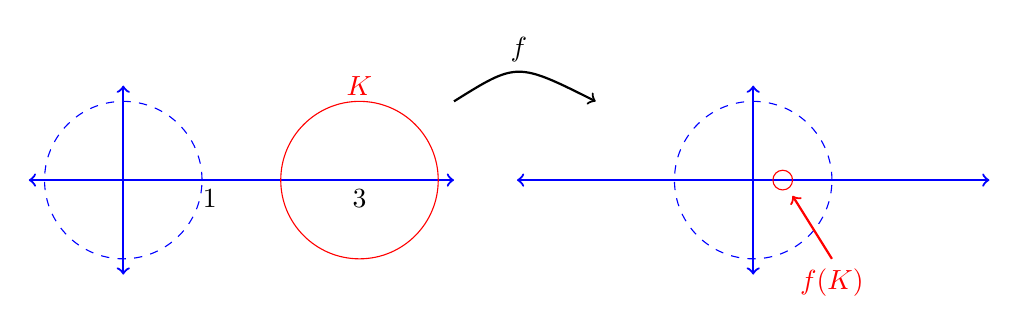
\begin{tikzpicture}
%left coordinate system
\draw[thick,blue,->] (0,0) -- (4.2,0);
\draw[thick,blue,->] (0,0) -- (0,1.2);
\draw[thick,blue,->] (0,0) -- (0,-1.2);
\draw[thick,blue,->] (0,0) -- (-1.2,0);
\node[below] at (1.1,0) {$1$};
\node[below] at (3,0) {$3$};
%circles
\draw[dashed,blue] (0,0) circle (1cm);
\draw[red] (3,0) circle (1cm);
\node[red] at (3,1.2) {$K$};
%arrow
\draw[thick,black,->] (4.2,1) .. controls (5,1.5) .. (6,1) node[pos=0.5,above] {$f$};
%right coordinate system
\draw[thick,blue,->] (8,0) -- (5,0);
\draw[thick,blue,->] (8,0) -- (11,0);
\draw[thick,blue,->] (8,0) -- (8,1.2);
\draw[thick,blue,->] (8,0) -- (8,-1.2);
%circles
\draw[dashed,blue] (8,0) circle (1cm);
\draw[red] (8.375,0) circle (0.125cm);
\draw[thick,red,->] (9,-1) -- (8.5,-0.2) node[pos=0,below] {$f(K)$};
\end{tikzpicture}
\end{figure}

\subsubsection{Facts About Mobius Transformations}
Every Mobius transformation maps circles and lines to circles or lines.\\
Given three distinct points $z_1, z_2, z_3 \in \hat{\mathbb{C}}$, there exists a unique Mobius transformation $f$ such that $f(z_1) = 0$, $f(z_2) = 1,$ and $f(z_3) = \infty$.\\
This transformation can be written down:
\begin{equation*}
f(z) = \frac{z - z_1}{z - z_3} \cdot \frac{z_2 - z_3}{z_2 - z_1}
\end{equation*}

\subsubsection{Further Facts}
\begin{itemize}
\item The composition of two Mobius transformations is a Mobius transformation, and so is the inverse.
\item Given three distinct points $z_1, z_2, z_3$ and three distinct points $w_1, w_2, w_3$, there exists a unique Mobius transformation $f : \hat{\mathbb{C}} \to \hat{\mathbb{C}}$ that maps $z_j$ to $w_j, j = 1, 2, 3$.
\begin{proof}
Let $f_1$ be the Mobius transformation that maps $z_1, z_2, z_3$ to $0, 1, \infty$.\\
Let $f_2$ be the Mobius transformation that maps $w_1, w_2, w_3$ to $0, 1, \infty$\\
Then $f_2^{-1} \circ f_1$ maps $z_1, z_2, z_3$ to $w_1, w_2, w_3$, respectively.
\end{proof}
\end{itemize}

\subsubsection{Compositions of Mobius transformations}
Every Mobius transformation is the composition of maps of the type
\begin{enumerate}
\item $z \longmapsto az$ (rotation and dilation)
\item $z \longmapsto z + b$ (translation)
\item $z \longmapsto \frac{1}{z}$ (inversion)
\end{enumerate}

\subsection{The Riemann Mapping Theorem}
\subsubsection{The Theorem}
What conformal mappings are there of the form $f : \mathbb{D} \to D$, where $\mathbb{D} = B_1(0)$ is the unit disk and $D \subset \mathbb{C}$?
\begin{theorem}
If $D$ is a simply connected domain (open, connected, no holes) in the complex plane, but not the entire complex plane, then there is a conformal map (analytic, one-to-one, onto) of $D$ onto the open unit disk $\mathbb{D}$.
\end{theorem}
\begin{figure}[h]
\centering
\includegraphics[scale=0.5]{Riemann_mapping_theorem.png}
\end{figure}

\section{Complex Integration}
\subsection{Complex Integration}
\subsubsection{The Fundamental Theorem of Calculus}
\begin{theorem}
Let $f : [a, b] \to \mathbb{R}$ be continuous, and define $F(x) = \int_a^x f(t)dt$. Then $F$ is differentiable and $F'(x) = f(x)$ for $x \in [a, b]$.
\end{theorem}

\subsubsection{Generalization to $\mathbb{C}$}
Integration in $\mathbb{C}$ is happening on curves.
\begin{equation*}
\gamma : [a, b] \to \mathbb{C}, \gamma (t) = x(t) + iy(t).
\end{equation*}
If $f$ is complex valued on $\gamma$, we define
\begin{equation*}
\int_{\gamma} f(z)dz = \lim_{n\to \infty} \sum_{j=0}^{n-1}f(z_j)(z_{j+1} - z_j)
\end{equation*}
where $z_j = \gamma (t_j)$ and $a = t_0 < t_1 < ... < t_n = b$. \\
It can be shown that if $\gamma : [a, b] \to \mathbb{C}$ is a smooth curve and $f$ is continuous on $\gamma$, then
\begin{equation*}
\int_{\gamma} f(z)dz = \int_a^b f(\gamma (t))\gamma '(t)dt
\end{equation*}
\begin{proof}
\begin{align*}
\sum_{j=0}^{n-1} f(z_j)(z_{j+1} - z_j) &= \sum_{j=0}^{n-1}f(\gamma (t_j))\frac{\gamma (t_{j+1}) - \gamma (t_j)}{t_{j+1} - t_j}(t_{j+1} - t_j) \\
&\to \int_a^b f(\gamma (t))\gamma '(t)dt \hspace{0.1cm} as \hspace{0.1cm} n \to \infty
\end{align*}
\end{proof}

\subsubsection{Independence of Parametrization}
Let $\gamma : [a, b] \to \mathbb{C}$ be a smooth curve, and let $\beta : [c, d] \to \mathbb{C}$ be another smooth parametrization of the same curve, given by $\beta (s) = \gamma (h(s))$, where $h :[c, d] \to [a, b]$ is a smooth bijection. \\
Let $f$ be a complex-valued function, defined on $\gamma$. Then
\begin{align*}
\int_{\beta} f(z)dz &= \int_c^d f(\beta (s))\beta '(s)ds \\
&= \int_c^d f(\gamma (h(s)))\gamma '(h(s)) h'(s)ds\\
&= \int_a^b f(\gamma (t))\gamma '(t)dt = \int_{\gamma} f(z)dz.
\end{align*}

\subsubsection{Piecewise Smooth Curves}
Let $\gamma = \gamma_1 + \gamma_2 + ... + \gamma_n$ be a piecewise smooth curve.\\
Then
\begin{equation*}
\int_{\gamma}f(z)dz = \int_{\gamma_1}f(z)dz + \int_{\gamma_2}f(z)dz + ... + \int_{\gamma_n}f(z)dz.
\end{equation*}
\begin{figure}[h]
\centering
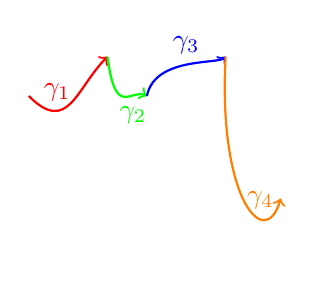
\begin{tikzpicture}
\draw[thick,red,->] (0,0) .. controls (0.5,-0.5) and (0.6,0.1) .. (1,0.5) node[pos=0.3, above] {$\gamma_1$};
\draw[thick,green,->] (1,0.5) .. controls (1.1,-0.3) and (1.3,0.1) .. (1.5,0) node[pos=0.7, below] {$\gamma_2$};
\draw[thick,blue,->] (1.5,0) .. controls (1.6, 0.5) and (2.4, 0.4) .. (2.5, 0.5) node[pos = 0.5, above] {$\gamma_3$};
\draw[thick,orange,->] (2.5, 0.5) .. controls (2.4, -1.3) and (3, -2) .. (3.2, -1.3) node[pos=0.7, above] {$\gamma_4$};
\end{tikzpicture}
\end{figure}

\subsubsection{Reverse Paths}
If $\gamma : [a, b] \to \mathbb{C}$ is a curve, then a curve $(-\gamma) : [a, b] \to \mathbb{C}$ is defined by 
\begin{equation*}
(-\gamma)(t) = \gamma(a + b - t).
\end{equation*}
If $f$ is continuous and complex-valued on $\gamma$, then
\begin{equation*}
\int_{(-\gamma)}f(z)dz = -\int_{\gamma}f(z)dz
\end{equation*}

\subsubsection{Linearity of the Path Integral}
If $\gamma$ is a curve, $c$ a complex constant and $f, g$ are continuous and complex-valued on $\gamma$, then
\begin{itemize}
\item $\int_{\gamma} (f(z) + g(z))dz = \int_{\gamma}f(z)dz + \int_{\gamma}g(z)dz$.
\item $\int_{\gamma}(cf)(z)dz = c \int_{\gamma}f(z)dz$.
\item $\int_{-\gamma}f(z)dz = - \int_{\gamma}f(z)dz$.
\end{itemize}

\subsubsection{Arc Length}
Given a curve $\gamma : [a, b] \to \mathbb{C}$, how can we find its length? \\
Let $a = t_0 < t_1 < ... < t_n = b.$ Then 
\begin{equation*}
length(\gamma) = \lim_{n \to \infty} \sum_{j=0}^{n} \left|\gamma (t_{j+1} - \gamma (t_j)\right|.
\end{equation*}
How to actually calculate this?
\begin{equation*}
\sum_{j=0}^{n}\left|\gamma(t_{j+1} - \gamma(t_j)\right| = \sum_{j=0}^{n} \frac{\left|\gamma(t_{j+1}) - \gamma(t_j)\right|}{t_{j+1} - t_j}(t_{j+1} - t_j) \to \int_a^b\left|\gamma '(t)\right|dt
\end{equation*}
Thus:
\begin{equation*}
length(\gamma) = \int_a^b \left|\gamma '(t)\right|dt.
\end{equation*}

\subsubsection{Integration With Respect To Arc Length}
\begin{definition}
Let $\gamma$ be a smooth curve, and let $f$ be a complex-valued and continuous function on $\gamma$. Then
\begin{equation*}
\int_{\gamma} f(z)\left|dz\right| = \int_a^b f(\gamma(t))\left|\gamma'(t)\right|dt
\end{equation*}
is the integral of $f$ over $\gamma$ with respect to arc length.
\end{definition}

\subsubsection{The ML-Estimate}
\begin{theorem}
If $\gamma$ is a curve and $f$ is continuous on $\gamma$ then
\begin{equation*}
\left|\int_{\gamma}f(z)dz\right| \leq \int_{\gamma}\left|f(z)\right|\left|dz\right|.
\end{equation*}
In particular, if $\left|f(z)\right| \leq M$ on $\gamma$, then
\begin{equation*}
\left|\int_{\gamma}f(z)dz\right| \leq M \cdot length(\gamma).
\end{equation*}
\end{theorem}

\subsection{The Fundamental Theorem of Calculus for Analytic Functions}
\subsubsection{Antiderivatives and Primitives}
\begin{definition}
If $f : [a, b] \to \mathbb{R}$ is continuous and has an antiderivative $F : [a, b] \to \mathbb{R}$, then
\begin{equation*}
\int_a^b f(x)dx = F(b) - F(a).
\end{equation*}
\end{definition}
Is there a complex equivalent?
\begin{definition}
Let $D \subset \mathbb{C}$ be a domain, and let $f : D \to \mathbb{C}$ be a continuous function. A primitive of $f$ on $D$ is an analytic function $F : D \to \mathbb{C}$ such that $F' = f$ on $D$.
\end{definition}

\subsubsection{Functions with Primitives}
\begin{theorem}
If $f$ is continuous on a domain $D$ and if $f$ has a primitive $F$ in $D$, then for any curve $\gamma : [a, b] \to D$ we have that
\begin{equation*}
\int_{\gamma}f(z)dz = F(\gamma(b)) - F(\gamma(a)).
\end{equation*}
\end{theorem}
\begin{remark}
\begin{itemize}
\item The integral only depends on the initial point and the terminal point of $\gamma$!
\item Big 'hidden' assumption: $f$ needs to have a primitive in $D$!
\end{itemize}
\end{remark}

\subsubsection{When Does $f$ Have a Primitive?}
\begin{theorem}[Goursat]
Let $D$ be a simply connected domain in $\mathbb{C}$, and let $f$ be analytic in $D$. Then $f$ has a primitive in $D$. Moreover, a primitive is given explicitly by picking $z_0 \in D$ and letting
\begin{equation*}
F(z) = \int_{z_0}^z f(w)dw.
\end{equation*}
where the integral is taken over an arbitrary curve in $D$ from $z_0$ to $z$.
\end{theorem}
One way to prove this theorem is as follows:
\begin{enumerate}
\item First, show Morera's Theorem: if $f$ is continuous on a simply connected domain $D$, and if $\int_{\gamma}f(z)dz = 0$ for any triangular curve $\gamma$ in $D$, then $f$ has a primitive in $D$.
\item Next, show the Cauchy Theorem for Triangles: for any triangle $T$ that fits into $D$ (including its boundary), $\int_{\partial T}f(z)dz = 0$.
\end{enumerate}

\subsubsection{The Cauchy Theorem for Triangles}
\begin{theorem}[Cauchy's Theorem for Triangles]
Let $D$ be an open set in $\mathbb{C}$, and let $f$ be analytic in $D$. Let $T$ be a triangle that fits into $D$ (including its boundary), and let $\partial T$ be its boundary, oriented positively. Then
\begin{equation*}
\int_{\partial T} f(z)dz = 0.
\end{equation*}
\end{theorem}
\begin{proof}
Assume
\begin{equation*}
\left|\int_{\partial T} f\right| = c \geq 0.
\end{equation*}
It will be shown that $c = 0$. \\
First, subdivide $T$ into four triangles, marked $T^1, T^2, T^3, T^4$ by joining the midpoints on the sides. Then it is true that
\begin{equation*}
\int_{\partial T} f = \sum_{r=1}^4 \left|\int_{T^r}f\right|
\end{equation*}
Choose $r$ such that
\begin{equation*}
\left| \int_{\partial T^r} f \right| \geq \frac{1}{4}c.
\end{equation*}
Defining $T^r$ as $T_1$, then
\begin{equation*}
\left| \int_{\partial T_1} f\right| \geq \frac{1}{4}c \hspace{0.1cm} and \hspace{0.1cm} L (\partial T_1) = \frac{1}{2} L(\partial T)
\end{equation*}
(where $L(\gamma)$ describes length of the curve). \\
Repeat this process of subdivision to get a sequence of triangles
\begin{equation*}
T \supset T_1 \supset T_2 \supset ... \supset ... T_n \supset ...
\end{equation*}
satisfying that 
\begin{equation*}
\left| \int_{\partial T_n} f\right| \geq (\frac{1}{4})^n c \hspace{0.1cm} and \hspace{0.1cm} L(\partial T_n) = (\frac{1}{2})^n L(\partial T).
\end{equation*}
Claim: The nested sequence $\overline{T} \supset \overline{T_1} \supset \overline{T_2} \supset ... \supset \overline{T_n} \supset ...$ contains a point $z_0 \in \cap_{n=1}^{\infty} \overline{T_n}$. On each step choose a point $z_n \in T_n$. Then it is easy to show that ($z_n$) is a Cauchy sequence. Then ($z_n$) converges to a point $z_0 \in \cap_{n=1}^{\infty} \overline{T_n}$ since each of the $\overline{T_n}$ are closed, hence, proving the claim. \\
We can generate another estimate of $c$ using the fact that $f$ is differentiable. Since $f$ is differentiable at $z_0$, for a given $\epsilon > 0$ there exists $\delta > 0$ such that
\begin{equation*}
0 < \left|z - z_0\right| < \delta \hspace{0.1cm} implies \hspace{0.1cm} \left| \frac{f(z) - f(z_0)}{z - z_0} - f'(z_0)\right| < \epsilon
\end{equation*}
which can be rewritten as
\begin{equation*}
0 < \left|z - z_0\right| < \delta \hspace{0.1cm} implies \hspace{0.1cm} \left|f(z) - f(z_0) - f'(z_0)(z - z_0)\right| < \epsilon \left|z -z_0\right|
\end{equation*}
For $z \in T_n$ we have $\left|z - z_0\right| < L(\partial)$, and so by the Estimation Lemma we have that
\begin{equation*}
\left| \int_{\partial T_n} \{f(z) - [f(z_0) + f'(z_0)(z - z_0)]\}dz \right| \leq \epsilon L^2(\partial)
\end{equation*}
As $f(z_0) + f'(z_0)(z - z_0)$ is of the form $\alpha z + \beta$ it has an antiderivative in $D$, and so $\int_{\partial T_n} f(z_0) + f'(z_0)(z - z_0) = 0$, and the above is then just
\begin{equation*}
\left| \int_{\partial T_n} f(z)dz \right| \leq \epsilon L^2(\partial)
\end{equation*}
Notice that 
\begin{equation*}
(\frac{1}{4})^n c \leq \left| \int_{\partial T_n} f(z)dz\right| \leq \epsilon L^2(\partial) = (\frac{1}{4})^n \epsilon L^2(\partial)
\end{equation*}
Giving
\begin{equation*}
c \leq \epsilon L^2(\partial).
\end{equation*}
Since $\epsilon > 0$ can be chosen arbitrary small, then $c = 0$.
\end{proof}

\subsubsection{Morera's Theorem}
\begin{theorem}[Morera's Theorem]
If $f$ is contiunous on a simply connected domain $D$, and if $\int_{\gamma}f(z)dz = 0$ for any triangular curve in $D$, then $f$ has a primitive in $D$.
\end{theorem}
\begin{proof}
Without loss of generality, it can be assumed that $D$ is connected. Fix a point $z_0$ in $D$, and for any $z \in D$, let $\gamma : [0, 1] \to D$ be a piecewise $C^1$ curve such that $\gamma(0) = z_0$ and $\gamma(1) = z$. Then define the function $F$ to be 
\begin{equation*}
F(z) = \int_{\gamma} f(\zeta)d\zeta.
\end{equation*}
To see that the function is well-defined, suppose $\tau : [0, 1] \to D$ is another piecewise $C^1$ curve such that $\tau(0) = z_0$ and $\tau(1) = z$. The curve $\gamma \tau^{-1}$ (i.e. the curve combining $\gamma$ with $\tau$ in reverse) is a closed piecewise $C^1$ curve in $D$. Then,
\begin{equation*}
\int_{\gamma} f(\zeta)d\zeta + \int_{\tau^{-1}} f(\zeta)d\zeta = \oint_{\gamma\tau^{-1}}f(\zeta)d\zeta = 0
\end{equation*}
And it follows that 
\begin{equation*}
\int_{\gamma} f(\zeta)d\zeta = \int_{\tau} f(\zeta)d\zeta.
\end{equation*}
Then using the continuity of $f$ to estimate difference quotients, we get that $F'(z) = f(z)$. Had we chosen a different $z_0$ in $D$, $F$ would change by a constant: namely, the result of integrating $f$ along any piecewise regular curve between the new $z_0$ and the old, and this does not change the derivative. \\
Since $f$ is the derivative of the holomorphic function $F$, it is holomorphic. The fact that derivatives of holomorphic functions are holomorphic can be proved by using the fact that holomorphic functions are analytic, i.e. can be represented by a convergent power series, and the fact that power series may be differentiated term by term. 
\end{proof}

\subsection{Cauchy's Theorem and Integral Formula}

\subsubsection{Cauchy's Theorem}
\begin{theorem}[Cauchy's Theorem for Simply Connected Domains]
Let $D$ be a simply connected domain in $\mathbb{C}$, and let $f$ be analytic in $D$. Let $\gamma : [a, b] \to D$ be apiecewise smooth, closed curve in D (i.e. $\gamma(b) = \gamma(a))$. Then
\begin{equation*}
\int_{\gamma}f(z)dz = 0.
\end{equation*}
\end{theorem}
\begin{proof}
If one assumes that the partial derivatives of a holomorphic function are continuous, the Cauchy integral theorem can be proved as a direct consequence of Green's theorem and the fact that the real and imaginary parts of $f = u + iv$ must satisfy the Cauchy-Riemann equations in the region bounded by $\gamma$, and moreover in the open neighbourhood $U$ of this region. Cauchy provided this proof, but it was later proved by Goursat without requiring techniques from vector calculus, or the continuity of partial derivatives.\\
We can break the integrand $f$, as well as the differential $dz$ into their real and imaginary components:
\begin{align*}
f &= u + iv \\
dz &= dx + i dy
\end{align*}
In this case we have
\begin{equation*}
\oint_{\gamma}f(z)dz = \oint_{\gamma}(u + iv)(dx + i dy) = \oint_{\gamma} (u dx - v dy) + i\oint_{\gamma} (v dx + u dy)
\end{equation*}
By Green's theorem, we may then replace the integrals around the closed contour $\gamma$ with an area integral throughout the domain $D$ that is enclosed by $\gamma$ as follows:
\begin{align*}
\oint_{\gamma} (u dx - v dy) &= \iint_D (-\frac{\partial v}{\partial x} - \frac{\partial u}{\partial y}) dx dy \\
\oint_{\gamma} (v dx + u dy) &= \iint_D (\frac{\partial u}{\partial x} - \frac{\partial v}{\partial y}) dx dy
\end{align*}
However, being the real and imaginary parts of a functionholomorphic in the domain $D$, $u$ and $v$ must satisfy the Cauchy-Riemann equations there:
\begin{align*}
\frac{\partial u}{\partial x} &= \frac{\partial v}{\partial y}\\
\frac{\partial u}{\partial y} &= -\frac{\partial v}{\partial x}
\end{align*}
We therefore find that both integrands (and hence their integrals) are zero
\begin{align*}
\iint_D (-\frac{\partial v}{\partial x} - \frac{\partial u}{\partial y}) dx dy &= \iint_D (\frac{\partial u}{\partial y} - \frac{\partial u}{\partial y}) dx dy = 0 \\
\iint_D (\frac{\partial u}{\partial x} - \frac{\partial v}{\partial y}) dx dy &= \iint_D (\frac{\partial u}{\partial x} - \frac{\partial u}{\partial x}) dx dy = 0
\end{align*}
This gives the desired result
\begin{equation*}
\oint_{\gamma} f(z)dz = 0
\end{equation*}
\end{proof}

\subsubsection{A first Conclusion of the Theorem}
\begin{corollary}
Let $\gamma_1$ and $\gamma_2$ be two simple closed curves (i.e. neither of the curves intersects itself), oriented counterclockwise, where $\gamma_2$ is inside $\gamma_1$. If $f$ is analytic in a domain $D$ that contains both curves as well as the region between them, then
\begin{equation*}
\int_{\gamma_1}f(z)dz = \int_{\gamma_2}f(z)dz.
\end{equation*}
\end{corollary}
\begin{proof}
Take the two curves and form a 'joint curve' $\gamma$ as in the picture below. As $f$ is analytic in a simply connected region, containing $\gamma$, we have $\int_{\gamma}f(z)dz = 0$.
\begin{figure}[h]
\centering
\includegraphics[scale=0.5]{Curves.png}
\end{figure}
\end{proof}

\subsubsection{The Cauchy Integral Formula}
\begin{theorem}[Cauchy Integral Formula]
Let $D$ be a simply connected domain, bounded by a piecewise smooth curve $\gamma$, and let $f$ be analytic in a set $U$ that contains the closure of $D$ (i.e. $D$ and $\gamma$). Then
\begin{equation*}
f(w) = \frac{1}{2\pi i} \int_{\gamma} \frac{f(z)}{z - w}dz
\end{equation*}
for all $w \in D$.
\end{theorem}
\begin{proof}
By using the Cauchy integral theorem, one can show that the integral over $C$ (or the closed rectifiable curve) is equal to the same integral taken over an arbitrarily small circle around $a$. Since $f(z)$ is continuous, we can choose a circle small enough on which $f(z)$ is arbitrarily close to $f(a)$. On the other hand, the integral
\begin{equation*}
\oint_{C} \frac{1}{z - a}dz = 2\pi i
\end{equation*}
over any circle centered at $a$. This can be calculated directly via a parametrization (integration by substitution) $z(t) = a + \epsilon e^{it}$ where $0 \leq t \leq 2\pi$ and $\epsilon$ is the radius of the circle. \\
Letting $\epsilon \to 0$ gives the desired estimate
\begin{align*}
\left| \frac{1}{2\pi i} \oint_{C} \frac{f(z)}{z-a}dz - f(a) \right| &= \left| \frac{1}{2\pi i}\oint_{C} \frac{f(z) - f(a)}{z - a}dz \right| \\
&= \left| \frac{1}{2\pi i} \int_0^{2\pi} (\frac{f(z(t)) - f(a)}{\epsilon e^{it}} \cdot \epsilon e^{it}i) dt \right| \\
&\leq \frac{1}{2\pi} \int_0^{2\pi} \frac{\left|f(z(t)) - f(a) \right|}{\epsilon} \epsilon dt \\
&\leq \max_{\left|z - a\right| = \epsilon} \left|f(z) - f(a)\right| \to 0 \hspace{0.1cm} as \hspace{0.1cm} \epsilon \to 0
\end{align*}
\end{proof}

\subsubsection{Analyticity of the Derivative}
\begin{theorem}
If $f$ is analytic in an open set $U$, then $f'$ is also analytic in $U$.
\end{theorem}
Idea of the proof:
\begin{itemize}
\item Use the Cauchy Integral Formula to show that for any $w \in U$, the derivative $f'(w)$ can be found via
\begin{equation*}
f'(w) = \frac{1}{2\pi i} \int_{\gamma} \frac{f(z)}{(z - w)^2}dz,
\end{equation*}
where $\gamma$ is the boundary of a small disk, centered at $w$; small enough so that it fits into $U$.
\item Next, show that the right-hand side defines an analytic function in $w$, and therefor $f'$ must be analytic.
\end{itemize}

\subsubsection{The Cauchy Integral Formula for Derivatives}
Repeated application of the previous theorem shows that an analytic function has infinitely many derivatives.
\begin{theorem}[Cauchy Integral Formula for Derivatives]
Let $D$ be a simply connected domain, bounded by a piecewise smooth curve $\gamma$, and let $f$ be analytic in a set $U$ that contains the closure of $D$ (i.e. $D$ and $\gamma$). Then
\begin{equation*}
f^{(k)}(w) = \frac{k!}{2\pi i} \int_{\gamma} \frac{f(z)}{(z - w)^{k+1}}dz \hspace{0.1cm} for \hspace{0.1cm} all \hspace{0.1cm} w \in D, k \geq 0.
\end{equation*}
\end{theorem}

\subsection{Consequences of Cauchy's Theorem and Integral Formula}

\subsubsection{Cauchy's Estimate}
\begin{theorem}
Suppose that $f$ is analytic in an open set that contains $\overline{B_r(z_0)}$, and that $\left|f(z)\right| \leq m$ holds on $\partial B_r(z_0)$ for some constant $m$. Then for all $k \geq 0$,
\begin{equation*}
\left|f^{(k)}(z_0)\right| \leq \frac{k!m}{r^k}.
\end{equation*}
\end{theorem}
\begin{proof}
By the Cauchy Integral Formula we have that
\begin{align*}
\left|f^{(k)}(z_0) \right| &= \frac{k!}{2\pi} \left| \int_{\left|z - z_0\right| = r} \frac{f(z)}{(z - z_0)^{(k+1)}}dz\right| \leq \frac{k!}{2\pi} \int_{\left|z - z_0\right|=r} \frac{\left|f(z)\right|}{\left|z - z_0\right|^{k+1}} \left|fz\right| \\
&\leq \frac{k!m}{2\pi r^{k+1}} \cdot 2\pi r = \frac{k!m}{r^k}.
\end{align*}
\end{proof}

\subsubsection{Liouville's Theorem}
\begin{theorem}[Liouville]
Let $f$ be analytic in the complex plane (thus $f$ is an entire function). If $f$ is bounded then $f$ must be constant.
\end{theorem}
\begin{proof}
Suppose that $\left|f(z)\right| \leq m$ for all $z \in \mathbb{C}$. Pick $z_0 \in \mathbb{C}$. Since $\mathbb{C}$ contains $\overline{B_r(z_0)}$ for any $r > 0$, we obtain from Cauchy's estimate:
\begin{equation*}
\left|f'(z_0)\right| \leq \frac{m}{r}
\end{equation*}
for any $r > 0$. Letting $r \to \infty$ we find that $f'(z_0) = 0$. Since $z_0$ was arbitrary, $f'(z) = 0$ for all $z$, hence $f$ is constant.
\end{proof}

\subsubsection{Use of Lioville's Theorem to Prove Fundamental Theorem of Algebra}
\begin{theorem}[Fundamental Theorem of Algebra]
Any polynomial $p(z) = a_0 + a_1z + ... + a_nz^n$ (with $a_0,...,a_n \in \mathbb{C}, n \geq 1$ and $a_n \neq 0$) has a zero in $\mathbb{C}$, i.e. there exists $z_0 \in \mathbb{C}$ such that $p(z_0) = 0$.
\end{theorem}
\begin{proof}
Suppose to the contrary that there exists a polynomial $p$ as in the theorem that has no zeros. Then $f(z) = \frac{1}{p(z)}$ is an entire function! Apply Liouville's theorem to $f$!
\begin{equation*}
p(z) = z^n(a_n + \frac{a_{n-1}}{z} + ... + \frac{a_0}{z^n})
\end{equation*}
, so
\begin{equation*}
\left|p(z)\right| \geq \left|z\right|^n (\left|a_n\right| - \frac{\left|a_{n-1}\right|}{\left|z\right|} - ... - \frac{\left|a_0\right|}{\left|z\right|^n}) \to \infty \hspace{0.1cm} as \hspace{0.1cm} \left|z\right| \to \infty.
\end{equation*}
Thus $\left|f(z)\right| \to 0$ as $\left|z\right| \to \infty$, and so $f$ is bounded in $\mathbb{C}$. By Liouville, $f$ is constant, and so $p$ is constant. This is a contradiction.
\end{proof}

\subsubsection{The Maximum Principle}
Another consequence of the Cauchy Integral Formula is
\begin{theorem}[Maximum Principle]
Let $f$ be analytic in a domain $D$ and suppose there exists a point $z_0 \in D$ such that $\left|f(z)\right| \leq \left|f(z_0)\right|$ for all $z \in D$. Then $f$ is constant in $D$.
\end{theorem}
\begin{remark}
If $D \subset \mathbb{C}$ is a bounded domain, and if $f : \overline{D} \to \mathbb{C}$ is continuous in $\overline{D}$ and analytic in $D$, then $\left|f\right|$ reaches its maximum on $\partial D$.
\end{remark}

\section{Power Series}

\subsection{Infinite Series of Complex Numbers}

\subsubsection{Infinite Series}
\begin{definition}
An infinite series
\begin{equation*}
\sum_{k=0}^{n} a_k = a_0 + a_1 + a_2 + ... + a_n + a_{n+1} + ...
\end{equation*}
(with $a_k \in \mathbb{C}$) converges to $S$ if the sequence of partial sums $\{S_n\}$, given by 
\begin{equation*}
S_n = \sum_{k=0}^{n}a_k = a_0 + a_1 + ... + a_n
\end{equation*}
converges to $S$.
\end{definition}

\begin{theorem}
If a series $\sum_{k=0}^{\infty} a_k$ converges then $a_k \to 0$ as $k \to \infty$.
\end{theorem}

\subsubsection{Absolute Convergence}
\begin{definition}
A series $\sum_{k=0}^{\infty} a_k$ converges absolutely if the series $\sum_{k=0}^{\infty}\left|a_k\right|$ converges.
\end{definition}
Examples:
\begin{itemize}
\item $\sum_{k=0}^{\infty} z^k$ converges and converges absolutely for $\left|z\right| < 1$.
\item $\sum_{k=1}^{\infty} \frac{i^k}{k}$ converges, but not absolutely.
\end{itemize}
\begin{theorem}
If $\sum_{k=0}^{\infty} a_k$ converges absolutely, then it also converges, and $\left|\sum_{k=0}^{\infty}a_k\right| \leq \sum_{k=0}^{\infty} \left|a_k\right|$.
\end{theorem}

\subsection{Power Series}
\subsubsection{Taylor Series}
\begin{definition}
A power series (also called Taylor series), centered at $z_0 \in \mathbb{C}$, is a series of the form
\begin{equation*}
\sum_{k=0}^{\infty} a_k(z - z_0)^k.
\end{equation*}
\end{definition}

\subsubsection{The Radius of Convergence}
\begin{theorem}
Let $\sum_{k=0}^{\infty}a_k(z - z_0)^k$ be a power series. Then there exists a number $R$, with $0 \leq R \leq \infty$, such that the series converges absolutely in $\{\left|z - z_0\right| < R \}$ and diverges in $\{\left|z - z_0\right| > R\}$. Furthermore, the convergence is uniform in $\{\left|z - z_0\right| \leq r\}$ for each $r < R$.
\end{theorem}

\subsubsection{Analyticity of Power Series}
\begin{theorem}
Suppose that $\sum_{k=0}^{\infty}a_k(z - z_0)^k$ is a power series of radius of convergence $R > 0$. Then
\begin{equation*}
f(z) = \sum_{k=0}^{\infty}a_k(z - z_0)^k \hspace{0.1cm} is \hspace{0.1cm} analytic \hspace{0.1cm} in \hspace{0.1cm} \{\left|z - z_0\right| < R \}
\end{equation*}
Furthermore, the series can be differentiated term by term, i.e.
\begin{equation*}
f'(z) = \sum_{k=1}^{\infty}a_k \cdot k(z - z_0)^{k-1}, f''(z) = \sum_{k=2}^{\infty}a_k \cdot k(k-1)(z - z_0)^{k-2},...
\end{equation*}
In particular, $f^{(k)}(z_0) = a_k \cdot k!$, i.e. $a_k = \frac{f^{(k)}(z_0)}{k!}$ for $k \geq 0$.
\end{theorem}

\subsubsection{Integration of Power Series}
If $\sum_{k=0}^{\infty}a_k(z - z_0)^k$ has radius of convergence $R$, then for any $w$ with $\left|w - z_0\right| < R$ we have that
\begin{equation*}
\int_{z_0}^{w} \sum_{k=0}^{\infty}a_k(z - z_0)^kdz = \sum_{k=0}^{\infty}a_k \int_{z_0}^{w} (z - z_0)^k dz = \sum_{k=0}^{\infty} a_k \frac{1}{k+1}(w - z_0)^{k+1}.
\end{equation*}
Here, the integral is taken over any curve in the disk $\{\left|z - z_0\right| < R \}$ from $z_0$ to $w$.

\subsection{The Radius of Convergence of a Power Series}

\subsubsection{The Ratio Test}
\begin{theorem}[Ratio Test]
If the sequence $\{ \left| \frac{a_k}{a_{k+1}}\right| \}$ has a limit as $k \to \infty$ then this limit is the radius of convergence, $R$, of the power series $\sum_{k=0}^{\infty}a_k(z-z_0)^k$.
\end{theorem}

\subsubsection{The Root Test}
\begin{theorem}[Root Test]
If the sequence $\{\sqrt[k]{\left|a_k\right|}\}$ has a limit as $k \to \infty$ then $R = \frac{1}{\lim_{k\to \infty}\{\sqrt[k]{\left|a_k\right|}\}}$.
\end{theorem}
\begin{remark}
\begin{itemize}
\item If $\lim_{k \to \infty} \{\sqrt[k]{\left|a_k\right|}\} = 0$ then $R = \infty$.
\item If $\lim_{k \to \infty} \{\sqrt[k]{\left|a_k\right|}\} = \infty$ then $R = 0$.
\end{itemize}
\end{remark}

\subsubsection{The Cauchy Hadamard Criterion}
\begin{theorem}
The radius of convergence of the power series $\sum_{k=0}^{\infty}a_k(z-z_0)^k$ equals
\begin{equation*}
R = \frac{1}{\lim_{k \to \infty} \sup \sqrt[k]{\left|a_k\right|}}.
\end{equation*}
\end{theorem}

\subsubsection{Analytic Functions And Power Series}
\begin{theorem}
Let $f : U \to \mathbb{C}$ be analytic and let $\{\left|z - z_0\right| < r \} \subset U$. Then in this disk, f has a power series representation
\begin{equation*} 
f(z) = \sum_{k=0}^{\infty} a_k (z - z_0)^k, \left|z - z_0\right| < r, where \hspace{0.1cm} a_k = \frac{f^{(k)}(z_0)}{k!}, k \geq 0.
\end{equation*}
The radius of convergence of this power series is $R \geq r$.
\end{theorem}
\begin{corollary}
If $f$ and $g$ are analytic in $\{\left|z - z_0\right| < r \}$ and if $f^{(k)}(z_0) = g^{(k)}(z_0)$ for all $k$, then $f(z) = g(z)$ for all $z$ in $\{\left|z - z_0\right| < r \}$.
\end{corollary}

\subsection{The Riemann Zeta Function And The Riemann Hypothesis}

\subsubsection{Introduction to the Zeta Function}
Recall:
\begin{equation*}
\sum_{n=1}^{\infty} \frac{1}{n} \hspace{0.1cm} diverges \hspace{0.1cm} (harmonic \hspace{0.1cm} series),
\end{equation*}
but
\begin{equation*}
\sum_{n=1}^{\infty} \frac{1}{n^s} \hspace{0.1cm} converges \hspace{0.1cm} for \hspace{0.1cm} all \hspace{0.1cm} s > 1.
\end{equation*}
This can be seen as follows:
\begin{align*}
\sum_{n=1}^{\infty} \frac{1}{n^s} \leq 1 + \int_1^{\infty} \frac{1}{x^s}dx &= 1 + \left. \frac{1}{1-s} \frac{1}{x^{s-1}} \right|_{1}^{\infty} \\
&= 1 - \frac{1}{1-s} \\
&= \frac{s}{s - 1} \hspace{0.1cm} (s > 1)
\end{align*}

\subsubsection{The Zeta Function}
Now consider $s \in \mathbb{C}$ instead of $s \in \mathbb{R}$.
\begin{definition}
For $s \in \mathbb{C}$ with $\Re (s) > 1$, the zeta function is defined as 
\begin{equation*}
\zeta (s) = \sum_{n=1}^{\infty} \frac{1}{n^s}.
\end{equation*}
\end{definition}
Note that for real $s$, we have that $n^s = e^{\ln n^s} = e^{s \ln n}$, so we define
\begin{equation*}
n^s = e^{s \log n} = e^{s \ln n} \hspace{0.1cm} for \hspace{0.1cm} s \in \mathbb{C}
\end{equation*}

\subsubsection{Convergence of $\zeta (s) = \sum_{n=1}^{\infty} \frac{1}{n^s}$}
Since $n^s = e^{s \ln n}$, we have that $\left|n^s\right| = \left| e^{s \ln n} \right| = e^{\Re (s) \ln n} = n^{\Re (s)}$. Thus
\begin{equation*}
\sum_{n=1}^{\infty} \left| \frac{1}{n^s}\right| = \sum_{n=1}^{\infty} \frac{1}{n^{\Re (s)(}},
\end{equation*}
and since $\Re (s) > 1$, the series on the right converges. Thus $\sum_{n=1}^{\infty} \frac{1}{n^s}$ converges absolutely in $\{ \Re (s) > 1 \}$. \\
In fact, the convergence is uniform in $\{ \Re (s) \geq r \}$ for any $r > 1$, and this can be used to show that $\zeta (s)$ is analytic in $\{ \Re (s) > 1 \}$.

\subsubsection{Analytic Continuation of the Zeta Function}
\begin{theorem}
The zeta function has an analytic continuation into $\mathbb{C} \setminus \{1\}$, and this continuation satisfies that $\zeta (s) \to \infty$ as $s \to 1$.
\end{theorem}
Slightly easier to construct is an extension to the right half plane $\{ \Re (s) > 0\}$, minus the point $1$, here is the outline: \\
\begin{equation*}
\sum_{n=1}^{N} \frac{1}{n^s} = \int_{1}^{N+1} \frac{1}{x^s}dx + \sum_{n=1}^{N}\delta_n (s),
\end{equation*}
where
\begin{equation*}
\delta_n (s) = \frac{1}{n^s} - \int_n^{n+1} \frac{1}{x^s}dx.
\end{equation*}
Observe that $\sum_{n=1}^{N} \delta_n(s)$ is analytic in $\{ \Re (s) > 0\}$. One can show that $\sum_{n=1}^{N}\delta_n(s)$ converges, as $N \to \infty$, to an analytic function $H(s)$ in $\{ \Re (s) > 0\}$. Thus
\begin{equation*}
\zeta (s) = \frac{1}{s-1} + H(s) \hspace{0.1cm} holds \hspace{0.1cm} for \hspace{0.1cm} \Re (s) > 1,
\end{equation*}
where $H(s)$ is analytic in $\{ \Re (s) > 0 \}$. We can therefore use this to define the zeta function in all of $\{ \Re (s) > 0 \} \setminus \{1\}$. This definition agrees with the original definition in $\{ \Re (s) > 1 \}$. 

\subsubsection{The Zeros of the Zeta Function}
Of much interest are the zeros of the zeta function, i.e. those $s \in \mathbb{C}$, for which $\zeta(s) = 0$. 
\begin{theorem}
The only zeros of the zeta funciton outside of the strip $\{ 0 \leq \Re (s) \leq 1 \}$ are at the negative even integers, $-2, -4, -6, ...$
\end{theorem}
\begin{itemize}
\item The zeros $-2, -4, -6, ...$ are often called the 'trivial zeros', and the region to be studied remains the strip $\{ \leq \Re (s) \leq 1 \}$.
\item A key result is that zeta has no zeros on the line $\{ \Re (s) = 1 \}$, this is an essential fact in the proof of the prime number theorem.
\item From the fact that zeta has no zeros on $\{ \Re (s) = 1 \}$ it can easily be deduced that it has no zeros on $\{ \Re (s) = 0 \}$ either, via a functional equation.
\end{itemize}

\subsubsection{The Riemann Hypothesis}
In his seminal paper in which he proved the analytic continuation of the zeta function to $\mathbb{C} \setminus \{1\}$, Riemann initiated important insights into the distribution of prime numbers. In this paper, he expressed his belief in the veracity of the following:
\begin{conjecture}[Riemann Hypothesis]
In the strip $\{ 0 < \Re (s) \ 1 \}$, all zeros of $\zeta$ are on the line $\{ \Re (s) = \frac{1}{2} \}$.
\end{conjecture}
Much research has been done in attempts to prove this conjecture:
\begin{itemize}
\item $\zeta(s)$ has infinitely many zeros in $\{ 0 < \Re (s) < 1 \}$.
\item The asymptotic distribution of the zeros of $\zeta$ in $\{ 0 < \Re (s) < 1 \}$ is known.
\item At least on third of the zeros in $\{ 0 < \Re (s) < 1 \}$ lie on the critical line $\{ \Re(s) = \frac{1}{2} \}$.
\item Trillions of zeros of zeta have been calculated - so far all of them lie on the critical line.
\item Numerical evidence and much research point to the validity of this conjecture, but it is to this day unproved and remains one of the most famous unsolved problems in mathematics.
\item The Riemann Hypothesis is on the list of seven 'Millennium Prize Problems' (declared by the Clay Mathematics Institute in 2000). Only one of these has been solved so far (as of summer 2013) - the so-called Poincare Conjecture (by Grigory Perelman).
\item The Riemann Hypothesis has strong implications on the distribution of prime numbers and on the growth of many other important arithmetic functions. It would greatly sharpen many number-theoretic results.
\end{itemize}

\subsection{The Prime Number Theorem}

\subsubsection{The Prime Counting Function}
\begin{definition}
Let $\pi(x) = $ number of primes less than or equal to $x$. This funciton is called the prime counting function.
\end{definition}
It is impossible to find an explicit formula fo $\pi(x)$, that's why we study the asymptotic behaviour of $\pi(x)$ as $x$ becomes very large.

\subsubsection{The Prime Number Theorem}
\begin{theorem}[Prime Number Theorem]
\begin{equation*}
\pi(x) \sim \frac{x}{\ln x} \hspace{0.1cm} as \hspace{0.1cm} x \to \infty.
\end{equation*}
\end{theorem}

\subsubsection{How is $\zeta(s)$ Related to Prime Numbers?}
\begin{align*}
\zeta(s) &= \frac{1}{1^s} + \frac{1}{2^s} + \frac{1}{3^s} + \frac{1}{4^s} + \frac{1}{5^s} + \frac{1}{6^s} + ... \\
&= (1 + \frac{1}{2^s} + \frac{1}{4^s} + \frac{1}{8^s} + ...)(1 + \frac{1}{3^s} + \frac{1}{9^s} + ...)(1 + \frac{1}{5^s} + \frac{1}{25^s} + ...)... \\
&= \prod_{p} \sum_{k=0}^{\infty} \frac{1}{p^{ks}} \\
&= \prod_{p} \frac{1}{1 - \frac{1}{p^s}}.
\end{align*}
Note:
\begin{itemize}
\item This product formula shows that $\zeta(s) \neq 0$ for $\Re(s) > 1$.
\item The key step in the proof of the prime number theorem is that $\zeta$ has no zeros on $\{ \Re(s) = 1\}$.
\item The prime number theorem says that $\pi(x) \sim \frac{x}{\ln x}$, but it doesn't have any information about the difference $\pi(x) - \frac{x}{\ln x}$.
\item However, the prime number theorem can also be written as $\pi(x) \sim Li(x)$, where $Li(x) = \int_2^x \frac{1}{\ln t}dt$ is the (offset) logarithmic integral function.
\item The proofs of the prime number theorem by Hadamard and de la Vallee Poussin actually show that $\pi(x) = Li(x) + $error term, where the error term grows to infinity at a controlled rate.
\item Van Koch (in 1901) was able to give the best possible bounds on the error term, assuming the Riemann hypothesis is true. Schoenfeld (in1976) made this precise and proved that the Riemann hypothesis is equivalent to 
\begin{equation*}
\left| \pi(x) - li(x)\right| < \frac{\sqrt{x} \ln x}{8\pi},
\end{equation*}
where $li(x) = \int_0^x \frac{1}{\ln t}dt$ is the (un-offset) logarithmic integral function, related to $Li(x)$ via $Li(x) = li(x) - li(2)$.
\end{itemize}
The veracity of the Riemann Hypothesis would therefore imply further results about the distribution of prime numbers, in particular, they'd be distributed beautifully regularly about 'expected' locations.

\section{Laurent Series and the Residue Theorem}

\subsection{Laurent Series}

\subsubsection{Review of Taylor Series}
If $f : U \to \mathbb{C}$ is analytic and $\{\left|z - z_0\right| < R \} \subset U$ then $f$ has a power series representation
\begin{equation*}
f(z) = \sum_{k=0}^{\infty} a_k(z - z_0)^k, \hspace{0.1cm} where \hspace{0.1cm} a_k = \frac{f^{(k)}(z_0)}{k!}, k \geq 0.
\end{equation*}

\subsubsection{Laurent Series Expansion}
\begin{theorem}
If $f : U \to \mathbb{C}$ is analytic and $\{r < \left|z - z_0 \right| < R \} \subset U$ then $f$ has a Laurent series expansion
\begin{equation*}
f(z) = \sum_{k=-\infty}^{\infty}a_k(z - z_0)^k = ... \frac{a_{-2}}{(z - z_0)^2} + \frac{a_{-1}}{(z - z_0)} + a_0 + a_1(z - z_0) + a_2(z - z_0)^2 + ...
\end{equation*}
that converges at each point of the annulus and coverges absolutely and uniformly in each sub annulus $\{s \leq \left|z - z_0\right| \leq t \}$, where $r < s < t <R$.
\end{theorem}

\subsubsection{The Coefficients $a_k$}
For a Laurent series 
\begin{equation*}
f(z) = \sum_{k=-\infty}^{\infty}a_k(z - z_0)^k, r < \left|z - z_0\right| < R
\end{equation*}
$f$ may not be defined at $z_0$, so we need a new approach.
\begin{equation*}
a_k = \frac{f^{(k)}(z_0)}{k!} =^{Cauchy} \frac{1}{2\pi i} \int_{\left|z - z_0\right| = s} \frac{f(z)}{(z - z_0)^{k+1}} dz
\end{equation*}
\begin{theorem}
If $f$ is analytic in $\{ r < \left|z - z_0\right| < R \}$, then
\begin{equation*}
f(z) = \sum_{k=-\infty}^{\infty} a_k(z - z_0)^k,
\end{equation*}
where
\begin{equation*}
a_k = \frac{1}{2\pi i} \int_{\left|z - z_0\right| = s} \frac{f(z)}{(z - z_0)^{k+1}}dz
\end{equation*}
for any $s$ between $r$ and $R$ and all $k \in \mathbb{Z}$.
\end{theorem}

\subsection{Isolated Singularities of Analytic Functions}

\subsubsection{Isolated Singularities}
\begin{definition}
A point $z_0$ is an isolated singularity of $f$ if $f$ is analytic in a punctured disk $\{0 < \left|z - z_0\right| < r \}$ centered at $z_0$.
\end{definition}
\begin{itemize}
\item $f(z) = \frac{1}{z}$ has an isolated singularity at $z_0 = 0$.
\item $f(z) = \frac{1}{\sin z}$ has isolated singularities at $z_0 = 0, \pm \pi, \pm 2\pi,...$
\item $f(z) = \sqrt{z}$ and $f(z) = \log z$ do not have isolated singularities at $z_0 = 0$ since these functions cannot be defined to be analytic in any punctured disk around $0$.
\item $f(z) = \frac{1}{z - 2}$ has an isolated singularity at $z_0 = 2$.
\end{itemize}

\subsubsection{Classification of Isolated Singularities}
\begin{definition}
Suppose $z_0$ is an isolated singularity of an analytic function $f$ with Laurent series $\sum_{k=-\infty}^{\infty} a_k(z - z_0)^k, 0 < \left|z - z_0\right| < r$. Then the singularity $z_0$ is
\begin{itemize}
\item removable if $a_k = 0$ for all $k < 0$.
\item a pole if there exists $N > 0$ so that $a_{N} \neq 0$ but $a_k = 0$ for all $k < -N$. The index $N$ is the order of the pole.
\item essential if $a_k \neq 0$ for infinitely many $k < 0$.
\end{itemize}
\end{definition}

\subsubsection{Removable Singularities}
Example: $f(z) = \frac{\sin z}{z} = 1 - \frac{z^2}{3!} + \frac{z^4}{5!} - ...$. The Laurent series looks like a Taylor series. Taylor series are analytic within their region of convergence. Thus, if we define $f(z)$ to have the value $1$ at $z_0 = 0$, then $f$ becomes analytic in $\mathbb{C}$: \\
$$
f(z) =  
\begin{cases} \frac{\sin z}{z}, &\mbox{if } z \neq 0 \\
1 &\mbox{if } z = 0 
\end{cases}
$$
The singularity has been removed.
\begin{theorem}[Riemann's Theorem]
Let $z_0$ be an isolated singularity of $f$. Then $z_0$ is a removable singularity if and only if $f$ is bounded near $z_0$.
\end{theorem}

\subsubsection{Poles}
\begin{theorem}
Let $z_0$ be an isolated singularity of $f$. Then $z_0$ is a pole if and only if $\left|f(z)\right| \to \infty$ as $z \to z_0$.
\end{theorem}
\begin{remark}
If $f(z)$ has a pole at $z_0$ then $\frac{1}{f(z)}$ has a removable singularity at $z_0$ (and vice versa).
\end{remark}

\subsubsection{Essential Singularities}
Example: $f(z) = e^{\frac{1}{z}} = \sum_{k=0}^{\infty} \frac{1}{k!} \frac{1}{z^k} = 1 + \frac{1}{z} + \frac{1}{2!} \frac{1}{z^2} + ...$ has an essential singularity at $z_0 = 0$.
\begin{theorem}[Casorati-Weierstraß]
Suppose that $z_0$ is an essential singularity of $f$. Then for every $w_0 \in \mathbb{C}$ there exists a sequence $\{ z_n \}$ with $z_n \to z_0$ such that $f(z_n) \to w_0$ as $n \to \infty$.
\end{theorem}

\subsubsection{Picard's Theorem}
\begin{theorem}[Picard]
Suppose that $z_0$ is an esential singularity of $f$. Then for every $w_0 \to \mathbb{C}$ with at most one exception there exists a sequence $\{ z_n \}$ with $z_n \to z_0$ such that $f(z_n) = w_0$.
\end{theorem}

\subsection{The Residue Theorem}

\subsubsection{Motivation}
Recall: $f$ has an isolated singularity at $z_0$ if $f$ is analytic in $\{ 0 < \left|z - z_0\right| < r \}$ for some $r > 0$. In that case, $f$ has a Laurent series expansion
\begin{equation*}
f(z) = \sum_{-\infty}^{\infty} a_k(z - z_0)^k, 0 < \left| z - z_0\right| < r.
\end{equation*}
Observe: if $0 < \rho < r$ then
\begin{equation*}
\int_{\left|z - z_0\right| = \rho} f(z)dz = \sum_{k=-\infty}^{\infty}a_k \int_{\left|z - z_0\right| = \rho} (z - z_0)^k dz.
\end{equation*}
What is $\int_{\left|z - z_0\right| = \rho} (z - z_0)^k dz$?
\begin{itemize}
\item For $k \neq -1$, the function $h(z) = (z - z_0)^k$ has a primitive, namely $H(z) = \frac{1}{k+1}(z - z_0)^{k+1}$. Therefore, $\int_{\left|z - z_0\right| = \rho} (z - z_0)^k dz = 0$ for $k \neq -1$.
\item For $k = -1$, the integral is $\int_{\left|z - z_0\right| = \rho} \frac{1}{z - z_0}dz$. We can use the Cauchy Integral Formula (or compute this directly) and find $\int_{\left|z - z_0\right| = \rho} (z - z_0)^k dz = 2\pi i$ for $k = -1$.
\end{itemize}
Hence 
\begin{equation*}
\int_{\left|z - z_0\right| = \rho} f(z)dz = \sum_{k=-\infty}^{\infty}a_k\int_{\left|z - z_0\right| = \rho}(z - z_0)^kdz = 2\pi i a_{-1}.
\end{equation*}
That is why $a_{-1}$ gets special attention.

\subsubsection{The Residue}
\begin{definition}
If $f$ has an isolated singularity at $z_0$ with Laurent series expansion
\begin{equation*}
f(z) = \sum_{k=-\infty}^{\infty}a_k(z - z_0)^k, 0 < \left|z - z_0\right| < r,
\end{equation*}
then the residue of $f$ at $z_0$ is $Res(f, z_0) = a_{-1}$.
\end{definition}

\subsubsection{The Residue Theorem}
\begin{theorem}[Residue Theorem]
Let $D$ be a simply connected domain, and let $f$ be analytic in $D$, except for isolated singularities. Let $C$ be a simple closed curve in $D$ (oriented counterclockwise), and let $z_1, ... , z_n$ be those isolated singularities of $f$ that lie inside of $C$. Then
\begin{equation*}
\int_{C}f(z)dz = 2\pi i \sum_{k=1}^n Res(f, z_k).
\end{equation*}
\end{theorem}

\subsection{Finding Residues}

\subsubsection{Residues at Removable Singularities}
$z_0$ is a removable singularity if $a_k = 0$ for all $k < 0$. In particular $a_{-1} = 0$ in that case, so that $Res(f, z_0) = 0$. \\
Example: 
\begin{align*}
f(z) = \frac{\sin z}{z} &= \frac{1}{z} \sum_{n=0}^{\infty} \frac{(-1)^n}{(2n + 1)!}z^{2n + 1} \\
&= 1 - \frac{1}{3!}z^2 + \frac{1}{5!}z^4 - ...
\end{align*}
Thus $Res(f, 0) = 0$.

\subsubsection{Residues at Simple Poles}
$z_0$ is a simple pole if $a_{-1} \neq 0$ and $a_k = 0$ for all $k \leq -1$.
\begin{equation*}
f(z) = \frac{a_{-1}}{z - z_0} + a_0 + a_1 (z - z_0) + a_2 (z - z_0)^2 + ... .
\end{equation*}
How to isolate $a_{-1}$? 
\begin{equation*}
(z - z_0)f(z) = a_{-1} + a_0(z - z_0) + a_1(z - z_0)^2 + ...,
\end{equation*}
so that
\begin{equation*}
Res(f, z_0) = a_{-1} = \lim_{z \to z_0} ((z - z_0)f(z))
\end{equation*}
Example: $f(z) = \frac{1}{z^2 + 1}$ has a simple pole at $z_0 = i$ (and another one at $-i$).
\begin{align*}
Res(\frac{1}{z^2+1},i) &= \lim_{z \to i}((z-i)\frac{1}{z^2+1}) \\
&= \lim_{z \to i} ((z-i)\frac{1}{(z-i)(z+i)}) \\
&= \lim_{z \to i} \frac{1}{z+i} = \frac{1}{2i} = -\frac{i}{2}.
\end{align*}

\subsubsection{Residues at Double Poles}
$z_0$ is a double pole if $a_{-2} \neq 0$ and $a_k = 0$ for all $k \leq -3$. \\
\begin{equation*}
f(z) = \frac{a_{-2}}{(z - z_0)^2} + \frac{a_{-1}}{z - z_0} + a_0 + a_1(z - z_0) + ...
\end{equation*}
How to isolate $a_{-1}$?
\begin{equation*}
(z-z_0)^2f(z) = a_{-2} + a_{-1}(z-z_0) + a_0(z - z_0)^2+...
\end{equation*}
so that
\begin{equation*}
\frac{d}{dz}((z-z_0)^2f(z)) = a_{-1} + 2a_0(z-z_0)+...
\end{equation*}
Hence
\begin{equation*}
Res(f,z_0) = a_{-1}= \lim_{z \to z_0} \frac{d}{dz}((z-z_0)^2f(z)).
\end{equation*}
Example: $f(z) = \frac{1}{(z-1)^2(z-3)}$ has a double pole at $z_0=1$ (and a simple one at $3$).
\begin{align*}
Res(\frac{1}{(z-1)^2(z-3)},1) &= \lim_{z \to 1} \frac{d}{dz}((z-1)^2 \frac{1}{(z-1)^2(z.3)}) \\
&= \lim_{z \to 1} \frac{-1}{(z-3)^2} = -\frac{1}{4}.
\end{align*}

\subsubsection{Residues at Poles of Order n}
$z_0$ is a pole of order $n$ if $a_{-n} \neq 0$ and $a_k = 0$ for all $k \leq -(n+1)$.
\begin{equation*}
f(z) = \frac{a_{-n}}{(z-z_0)^n} + ... + \frac{a_{-1}}{z-z_0} + a_0 + a_1(z-z_0) + ...
\end{equation*}
Then
\begin{equation*}
Res(f,z_0) = a_{-1} = \frac{1}{(n-1)!} \lim_{z \to z_0} \frac{d^{n-1}}{dz^{n-1}}((z-z_0)^nf(z)).
\end{equation*}

\subsubsection{More on Residues}
\begin{remark}
If $f(z) = \frac{g(z)}{h(z)}$, where $g$ and $h$ are analytic near $z_0$, and $h$ has a simple zero at $z_0$, then
\begin{equation*}
Res(f(z),z_0) = \frac{g(z_0)}{h'(z_0)}
\end{equation*}
\end{remark}

\subsection{Evaluating Integrals via the Residue Theorem}
Example: \\
$\int_{\left|z\right| = 1} e^{\frac{3}{z}}dz = 2\pi i Res(f,0)$, where $f(z) = e^{\frac{3}{z}} = \sum_{k=0}^{\infty} \frac{1}{k!}(\frac{3}{z})^k$. Thus $Res(f,0) = 3$, so that
\begin{equation*}
\int_{\left|z\right| = 1} e^{\frac{3}{z}}dz = 6\pi i.
\end{equation*}

\subsubsection{More Examples}
The Residue Theorem can also be used to evaluate real integrals, for example of the following forms:
\begin{itemize}
\item $\int_0^{2\pi} R(\cos t, \sin t) dt$, where $R(x,y)$ is a rational function of the real variables $x$ and $y$.
\item $\int_{-\infty}^{\infty}f(x)dx$, where $f$ is a rational function of $x$.
\item $\int_{-\infty}^{\infty}f(x)\cos (\alpha x)dx$, where $f$ is a rational function of $x$.
\item $\int_{-\infty}^{\infty}f(x)\sin (\alpha x)dx$, where $f$ is a rational function of $x$.
\end{itemize}

\subsection{Evaluating an Improper Integral via the Residue Theorem}

\subsubsection{An Improper Integral}
Evaluate $\int_0^{\infty} \frac{\cos x}{1 + x^2}dx$. \\
Idea: 
\begin{align*}
\int_0^R \frac{\cos x}{1 + x^2} dx &= \frac{1}{2} \int_{-R}^R \frac{\cos x}{1 + x^2}dx \\
&= \frac{1}{2} \int_{-R}^{R} \frac{\cos x + i \sin x}{1 + x^2}dx \\
&= \frac{1}{2} \int_{-R}^{R} \frac{e^{ix}}{1 + x^2}dx.
\end{align*}

\begin{figure}[h]
\centering
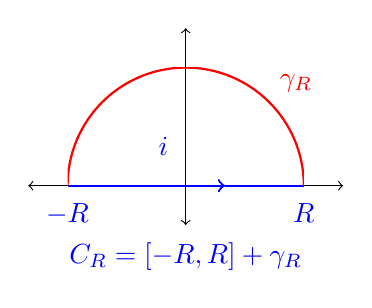
\begin{tikzpicture}
\draw[black,->] (0,0) -- (2,0);
\draw[black,->] (0,0) -- (-2,0);
\draw[black,->] (0,0) -- (0,2);
\draw[black,->] (0,0) -- (0,-0.5);

\draw[thick,blue,->] (-1.5,0) -- (0.5,0);
\draw[thick,blue] (0.5, 0) -- (1.5,0);

\begin{scope}
	\clip (-1.5,0) rectangle (1.5,1.5);
	\draw[thick,red] (0,0) circle(1.5);
\end{scope}
\node[below = 1mm of {(-1.5,0)}, blue] {$-R$};
\node[below = 1mm of {(1.5,0)}, blue] {$R$};
\node[below = 1mm of {(0,-0.5)}, blue] {$C_R = [-R, R] + \gamma_R$};
\node[left = 1mm of {(0,0.5)}, blue] {$i$};
\node[above right = 1mm of {(1,1)},red] {$\gamma_R$};
\end{tikzpicture}
\end{figure}

\begin{align*}
\frac{1}{2}\int_{-R}^{R}\frac{e^{ix}}{1 + x^2} dx &= \frac{1}{2} \int_{[-R,R]} \frac{e^{iz}}{1 + z^2}dz \\
&= \frac{1}{2} \int_{C_R} \frac{e^{iz}}{1 + z^2}dz - \frac{1}{2} \int_{\gamma_R} \frac{e^{iz}}{1 + z^2}dz \\
&= \frac{1}{2} \cdot 2\pi i Res(\frac{e^{iz}}{1+z^2},i) - \frac{1}{2} \int_{\gamma_R} \frac{e^{iz}}{1+z^2}dz.
\end{align*}
We thus need to find the residue of $f(z) = \frac{e^{iz}}{1+z^2}$ at $z_0 = i$ and estimate the integral over $\gamma_R$.

\begin{enumerate}
\item Finding the residue of $f(z) = \frac{e^{iz}}{1+z^2}$ at $z_0= i$:
\begin{itemize}
\item $f$ has a simple pole at $z = 0$.
\item Thus $Res(f,i) = \lim_{z \to i} (z-i)f(z) = \lim_{z \to i} \frac{(z-i)e^{iz}}{1+z^2} = \lim_{z \to i} \frac{e^{iz}}{z + i} = \frac{e^{-1}}{2i}$.
\item Hence $\frac{1}{2} \int_{C_R} \frac{e^{iz}}{1+z^2}dz = \frac{1}{2}2\pi i\frac{1}{2ie} = \frac{\pi}{2e}$.
\end{itemize}
\item Estimating $\frac{1}{2} \int_{\gamma_R}\frac{e^{iz}}{1+z^2}dz$:
\begin{itemize}
\item We are only interested in what happens as $R \to \infty$.
\item Want to show: $\frac{1}{2} \int_{\gamma_R} \frac{e^{iz}}{1+z^2}dz \to 0$ as $R \to \infty$.
\item Therefore, it suffices to show that $\left|\int_{\gamma_R} \frac{e^{iz}}{1+z^2}dz\right| \leq const(R)$, where the constant goes to zero as $R \to \infty$.
\item $\left|\int_{\gamma_R}f(z)dz\right| \leq length(\gamma_R) \cdot \max_{z \in \gamma_R} \left|f(z)\right|$.
\item $\left| \frac{e^{iz}}{1+z^2}\right| = \frac{e^{\Re (iz)}}{\left|1+z^2\right|} = \frac{e^{-y}}{\left|1+z^2\right|} \leq \frac{e^{-y}}{R^2-1} \leq \frac{1}{R^2-1}$ for $z \in \gamma_R$, since $\left|z\right| = R$ and $y \geq 0$ on $\gamma_R$.
\item $\left|\int_{\gamma_R} \frac{e^{iz}}{1+z^2}dz\right| \leq \pi R \cdot \frac{1}{R^2 - 1} \to 0$ as $R \to \infty$.
\item Thus $\int_{\gamma_R} \frac{e^{iz}}{1+z^2}dz \to 0$ as $R \to \infty$.
\end{itemize}
\end{enumerate}
Conclusion \\
To find $\int_0^{\infty} \frac{\cos x}{1+x^2}dx$ here is what we have:
\begin{enumerate}
\item \begin{equation*} \int_0^{\infty} \frac{\cos x}{1+x^2}dx = \lim_{R \to \infty} \int_0^R \frac{\cos x}{1+x^2}dx\end{equation*}
\item \begin{equation*} \int_0^R \frac{\cos x}{1+x^2}dx = \frac{1}{2} \int_{C_R} \frac{e^{iz}}{1+z^2}dz - \frac{1}{2} \int_{\gamma_R} \frac{e^{iz}}{1+z^2}dz \end{equation*}
\item \begin{equation*} \frac{1}{2} \int_{C_R} \frac{e^{iz}}{1+z^2}dz = \frac{1}{2} \cdot 2 \pi i Res(\frac{e^{iz}}{1+z^2},i) = \frac{\pi}{2e} \end{equation*}
\item \begin{equation*} \int_{\gamma_R} \frac{e^{iz}}{1+z^2}dz \to 0 \hspace{0.1cm} as \hspace{0.1cm} R \to \infty. \end{equation*}
\end{enumerate}
Hence $\int_0^{\infty} \frac{\cos x}{1+x^2}dx = \frac{\pi}{2e}$.


\end{document}